\chapter{Representative numerical simulations -- I}
\label{numerical-simulations-1}

Stemming in no small part from the physical richness of the system
under consideration, the theoretical formulation presented in the
preceding chapter resulted in a set of coupled, nonlinear partial
differential equations governing the interrelated mechanical and
biochemical processes underlying biological tissue growth.

In this chapter, a finite element implementation employing a staggered
scheme is used to solve this system of equations for a varied class of
numerical examples which aim to demonstrate the applicability of the
theory, and study aspects of the coupled phenomena as the tissue
grows. In Section~\ref{computational-model}, the numerical methods
used for coupling reaction, transport and mechanics are outlined, and
the computational model used in the simulations is introduced. The
opening example, presented in Section~\ref{enzyme-kinetics-example},
incorporates all of the theory discussed and acts as a model for
localised, bolus delivery of regulatory chemicals to tendons while
accounting for mechanical effects. In order to suppress some of the
coupled phenomena, and take a closer look at the physics of porous
soft tissues, Section~\ref{biphasic-examples-1} considers some
examples based on a simplified system comprising only of a solid phase
and a fluid phase. The final example presented in this chapter
provides a straightforward extension of the theory to model the
effects of the mechanical environment on wound healing
(Section~\ref{wound-healing-example}), evidencing the generality of
the proposed formulation.

\section{Introducing the computational model}
\label{computational-model}

The mathematical formulation developed in Sections~\ref{balance-laws}%
--\ref{algorithmic-considerations} has been implemented in a finite
element setting using {\tt FEAP} \citep{FEAPmanual}, a general purpose
nonlinear finite element program. The implementation is in
three-dimensions and uses eight-noded hexahedral elements.

The mass balance equation (\ref{current-mass-balance}) for
\mbox{$\iota = \mathrm{f}$} is solved to determine the current
concentration field of the fluid phase,\footnote{Recall from
  Section~\ref{role-of-current-mass-balance} that the physics of
  fluid-tissue interactions and the imposition of relevant boundary
  conditions are best understood and represented in the current
  configuration.} $\rho^{\mathrm{f}}$. The current
concentration of the solute, $\rho^{\mathrm{s}}$, is determined from
the stabilised form of the mass balance equation provided in weak form
in (\ref{stabilizedmassbal}). The mass balance for the solid phase is
solved in the reference configuration
(Equation~(\ref{localbalanceofmass}) for \mbox{$\iota = \mathrm{c}$}) to
obtain the concentration field, $\rho_{0}^{\mathrm{s}}$, since there
are no boundary conditions associated with this differential
equation. Backward Euler is used as the time-stepping scheme for these
equations.

In the implementation presented in this chapter, the tissue is viewed
as a single entity when imposing the balance of momentum; and a
summation of Equation~(\ref{localbalanceofmomentum}) over
$\iota=\mathrm{c,f}$ is solved using the relation
(\ref{momentumsummationresult}) for the common displacement
\mbox{field, $\bu$,} of the tissue and the fluid-filled
pores.\footnote{The ramifications of this simplification are
  explored in Section~\ref{constriction-1}.} Non-linear projection
methods \citep{simotaylorpister:85} based on hexahedral elements are
used to treat the near-incompressibility imposed by the fluid, and
mixed methods, as described in \cite{Garikipatiox2:01}, are used for
stress (and strain) gradient driven fluxes. Since the time scale for
mass transport is much larger than that for mechanics, and since we
are not focusing on inertial effects for the growth problems presented
in this chapter, the momentum equation is solved as a quasi-static
problem.\footnote{The numerical experiments presented in
  Section~\ref{biphasic-examples-2} contrast the results obtained from
  quasi-static and dynamic calculations.}

The coupling between mass transport and mechanics is achieved by an
iterative operator-splitting algorithm
\citep{Armero-poroplasticity:99, Garikipatietal:01}. Illustratively,
in the simplest case of a biphasic problem involving no
interconversion between species, this algorithm, in explicit terms,
reads:

\begin{itemize}
\item[] {\tt At each time step, repeat:}
  \begin{itemize}
  \item[$\circ$] {\tt Fix the fluid concentration field; solve the
    mechanics\\ problem for the displacement field,} $\bu$
  \item[$\circ$] {\tt Fix the displacement field; solve the
    mass-transport\\ problem for the concentration field,} $\rho^f$
  \end{itemize}
\item[]{\tt until both problems converge.}
\end{itemize}

\noindent Its generalisation to other cases involving additional differential
equations is straightforward.

The model geometry, based on the experimental work of \citet{Calve:04}
on the engineering and characterisation of tendon-like constructs (see
Figure~\ref{engconst}), is a cylinder 12 mm in length and 1 mm$^2$ in
cross-sectional area. The corresponding finite element mesh using 3840
hexahedral elements is shown in Figure~\ref{egmesh}. The constitutive
relation for the solid collagen uses a strain energy arising from the
eight-chain model incorporating worm-like chains discussed in
Section~\ref{anisotropic-network-elasticity} . The constitutive
relation for the (ideal) fluid stress follows (\ref{Pf}) with,

\begin{figure}[ht]
\centering
  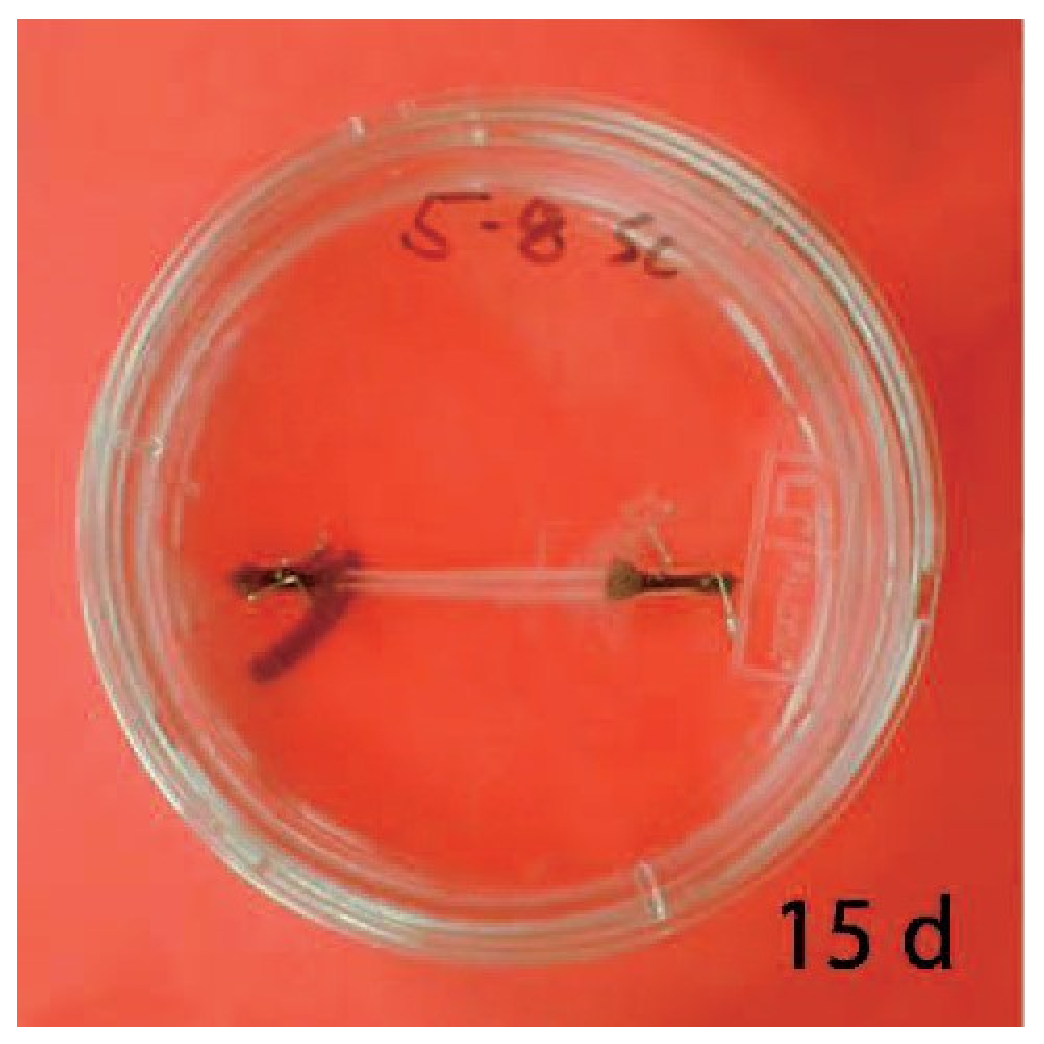
\includegraphics[width=0.6\textwidth]{images/experiments/one-construct}
\caption{Engineered tendon construct. See \citet{Calve:04} for
  details.} 
\label{engconst}
\end{figure}

\begin{figure}[ht]
  \centering
  \psfrag{D}{\small$1.1284$ mm}
  \psfrag{H}{\small$12.0$ mm}
  {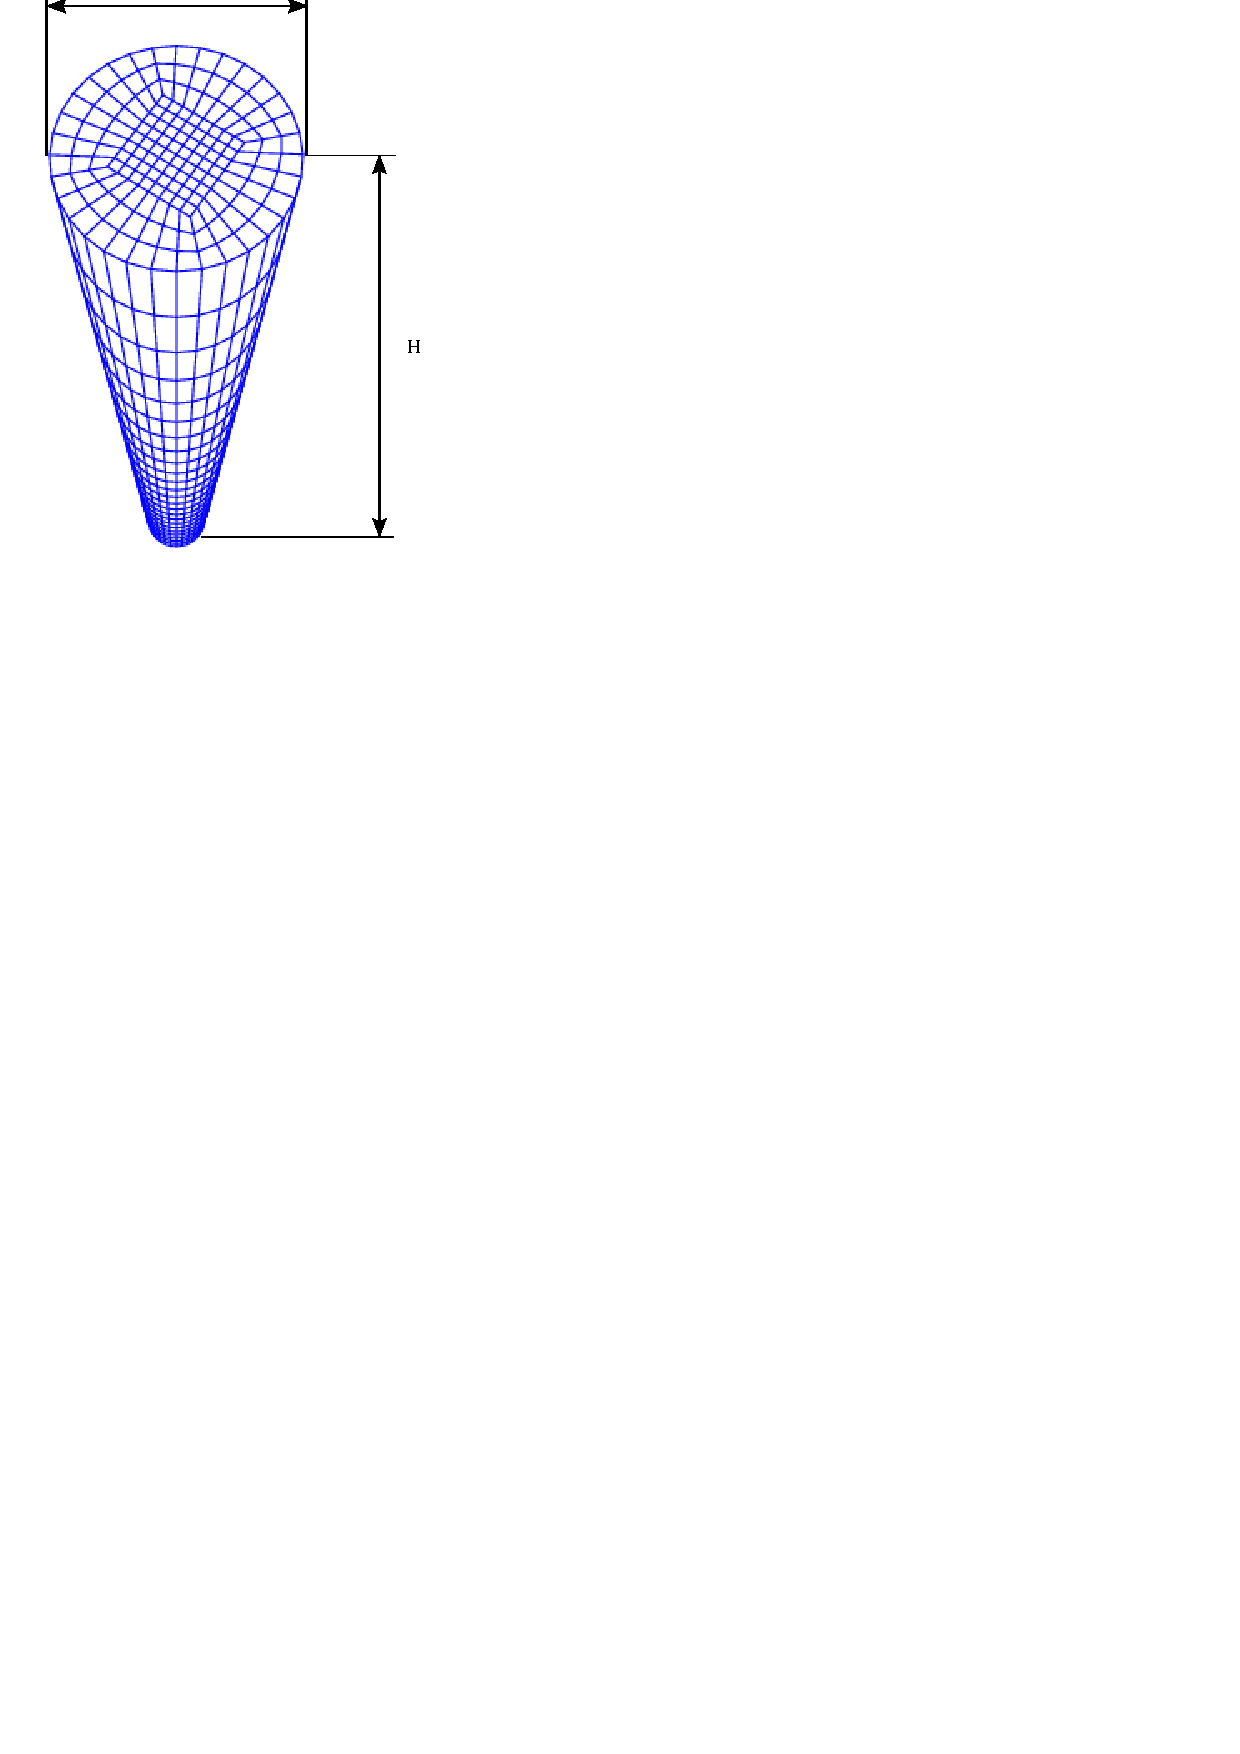
\includegraphics[width=0.4\textwidth]{images/examples/lagrangian/mesh}}
  \caption{The finite element mesh used in the computations.}
  \label{egmesh}
\end{figure}

\begin{equation}
h(\rho^\mathrm{f}) =
\frac{1}{2}\kappa^\mathrm{f}\left(
\frac{\rho_{0_\mathrm{ini}}^\mathrm{f}}{\rho^\mathrm{f}}
- 1\right)^2,
\end{equation}

\noindent where $\kappa^\mathrm{f}$ is the bulk modulus of the fluid.

The tissue is modelled as being fluid saturated in $\Omega_t$ at $t =
0$, i.e. (\ref{saturation}$_1$) holds with
$\rho^\mathrm{f}_{0_\mathrm{sat}} =
\rho^\mathrm{f}_{0_\mathrm{ini}}$. However, the tissue is allowed to
become unsaturated in $\Omega_t$ for $t > 0$ due to void
formation. Then, the conditions set out in (\ref{cavitation})
apply. The chemical potential is then given by
(\ref{fickeanmobility}). The numerical examples that follow discuss
further specialisation of the constitutive relations to relevant
cases.

The initial and boundary conditions have been chosen in order to model
a few common mechanical and chemical interventions on engineered
tissue and the numerical values of parameters\footnote{The mobility
  tensor reported in Table~\ref{parameters} is an order-of-magnitude
  estimate recalculated from \citet{Hanetal:2000} to correspond to the
  mobility used in this work. These authors reported a mean value of
  $0.927\times 10^{-14}$ s, with a range of $1.14\times
  10^{-14}--0.58\times 10^{-14}$ s in terms of the mobility used
  here. Theirs is the mobility parallel to the fibre direction in
  Rabbit Achilles tendon. Here, it is used as an isotropic
  mobility. Using anisotropic mobilities, or different values from the
  reported range changes the result quantitatively, but not
  qualitatively.} that have been used are relevant to tendons and
appear in Table~\ref{parameters}.

\section{A multiphasic problem based on enzyme-kinetics}
\label{enzyme-kinetics-example}

\begin{table}
\centering
\begin{tabular}{lll}
\hline \multicolumn{1}{c}{Parameter (Symbol)} & Value & Units\\ \hline
Chain density ($N$) & $7\times 10^{21}$ &
$\mathrm{m}^{-3}$\\ Temperature ($\theta$) & $310.6$ & K\\ Persistence
length ($A$) & $2.10$ & --\\ Fully-stretched length ($L$) & $2.125$ &
--\\ Unit cell axes ($a,\;b,\;c$) & $1.95,\;1.95,\;2.43$ & --\\ Bulk
compressibility factors ($\gamma,\;\beta$) & $1000,\; 4.5$ &
--\\ Fluid bulk modulus ($\kappa^f$) & $1$ & GPa\\ Fluid mobility
tensor ($D^\mathrm{f}_{ij} = D^\mathrm{f}\delta_{ij}$) & $1\times
10^{-14}$ &s\\
Fibroblast concentration ($\rho_{\mathrm{cell}}$) & 0.2 &
kg.m$^{-3}$\\ Max. reaction rate ($k_{\mathrm{max}} = 5$) & 5 &
s$^{-1}$\\ Max. solute concentration ($\rho^{\mathrm{s}}_m$) & 0.2 &
kg.m$^{-3}$\\ Solute diffusivity ($\bD^\mathrm{s}$) & $1\times
10^{-9}$ & m$^{-2}$s\\ \hline
\end{tabular}
\caption{Material parameters used in the analysis.}
\label{parameters}
\end{table}

This first example can be viewed as a model for localised, bolus
delivery of regulatory chemicals to the tendon while accounting for
mechanical (stress) effects. A single solute species\footnote{Here, we
  envision the solute to be a protein playing an essential role in
  growth by catalysing underlying biochemical reactions. An important
  example of this is a family of proteins, TGF$\beta$, which is a
  multi-functional peptide that controls numerous functions of many
  cell types \citep{Alberts:02}.} is considered, denoted by s, and a
uniform distribution of fibroblasts that are characterised by their
cell concentration, $\rho_{\mathrm{cell}}$. Both, Fickean diffusion of
the solute, and stress gradient driven fluid flow are incorporated in
this illustration. Michaelis-Menten enzyme kinetics
(\ref{enzyme-kinetics-source}) is used to determine the rates of
solute consumption and collagen production as a function of solute
concentration. This non-linear relationship for our choice of
parameters is visualised in Figure~\ref{eg3menten}. Here, the fluid
phase does not take part in reactions, and hence $\Pi^\mathrm{f}=0$.

\begin{figure}[!hpt]
  \centering
  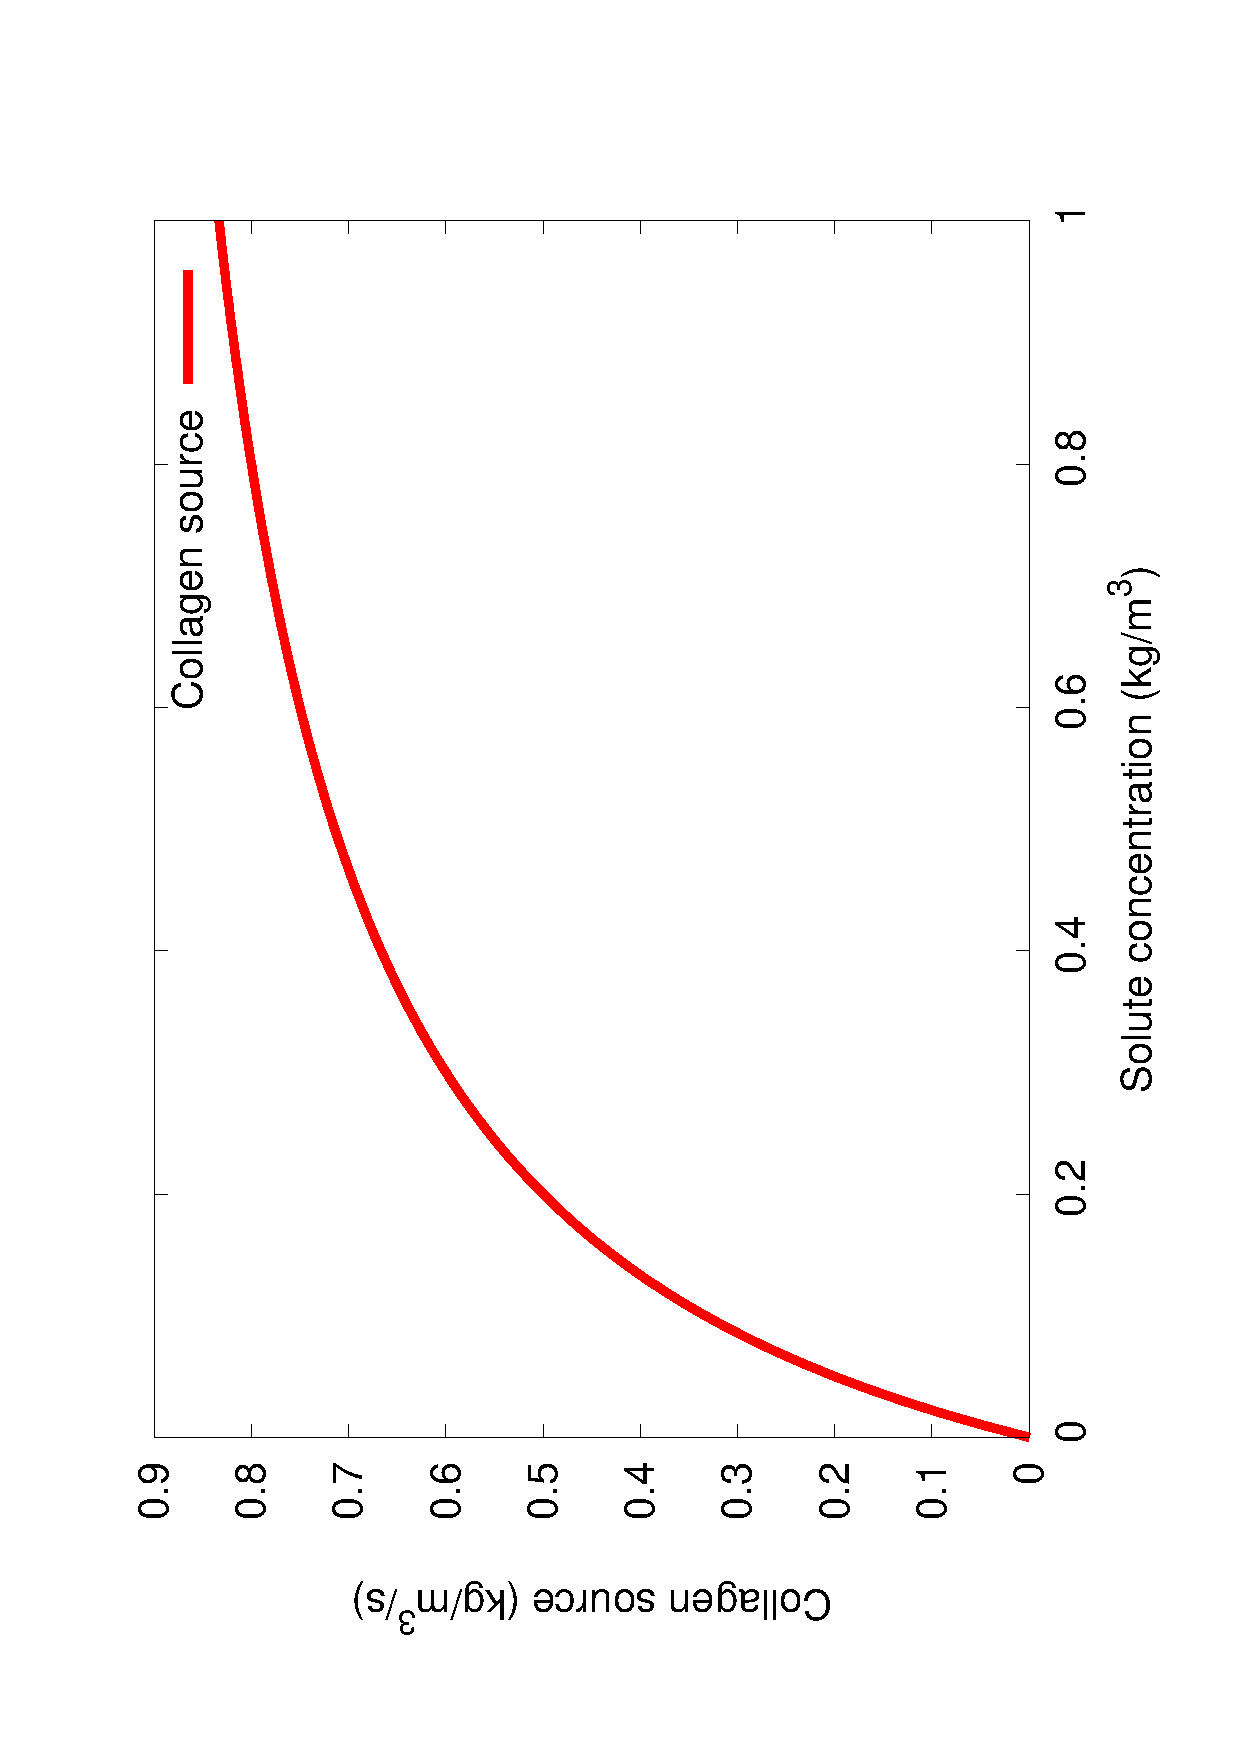
\includegraphics[angle=270,width=0.8\textwidth]{images/elucidation/enzyme-kinetics}
  \caption{Variation of the collagen source with solute
    concentration.}
  \label{eg3menten}
\end{figure}

The tendon immersed in the bath is subjected to a constrictive radial
load, such as would be imposed upon manipulating it with a set of
tweezers, as depicted in Figure~\ref{constrictload}. The maximum
strain in the radial direction---experienced half-way through the
height of the tendon---is 10\%. The applied strain in the radial
direction decreases linearly with distance from the central plane, and
vanishes at the top and bottom surfaces of the tendon.


\begin{figure}[!hpt]
  \centering
  \psfrag{M}{\small $\bN\cdot\bM^f$}
  \psfrag{P}{\small ${\tiny\quad }~\bu$}
  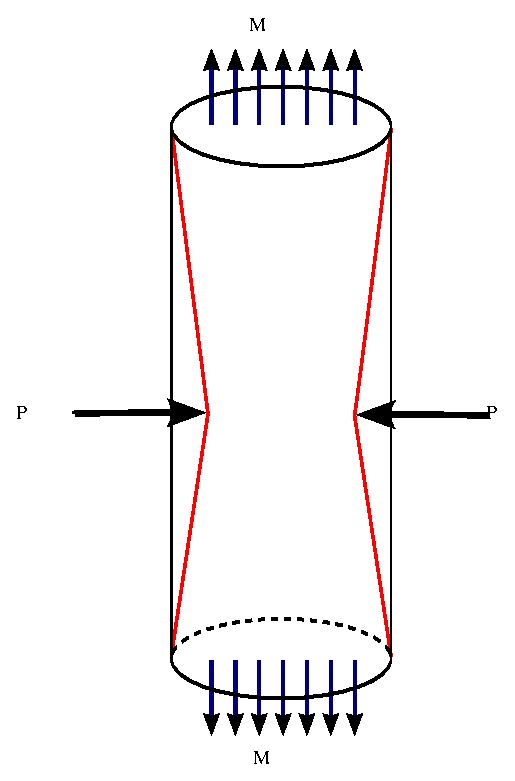
\includegraphics[width=5.0cm]{images/examples/lagrangian/constriction/cylinder-in-bath}
  \caption{Constrictive load applied to tendon immersed in a bath.}
  \label{constrictload}
\end{figure}

The initial collagen concentration and the initial fluid concentration
are both 500~kg.m$^{-3}$ at every point in the tendon, and the fluid
concentration in the bath is 500~kg.m$^{-3}$. In addition, a
solute-rich bulb of radius 0.15~mm is introduced with its centre on
the axis of the tendon and situated 3~mm below the upper circular face
of the tendon. The initial solute concentration is 0.05~kg.m$^{-3}$ at
all other points in the tendon, and increases linearly with decreasing
radius in this bulb to 1~kg.m$^{-3}$ at its centre (see
Figure~\ref{eg3ini}).

\begin{figure}[!hpt]
\centering
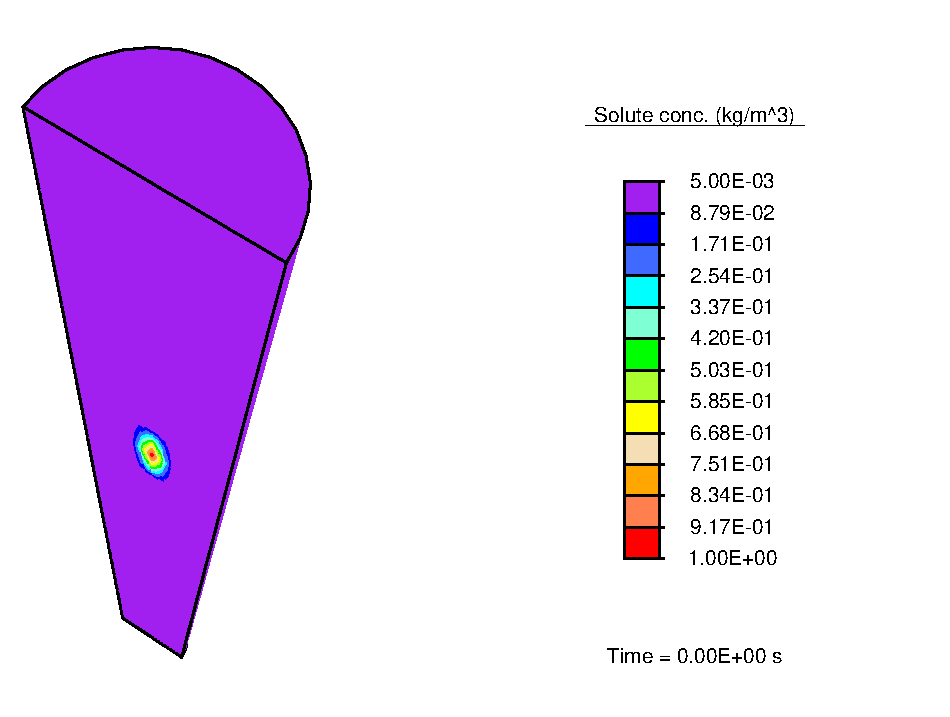
\includegraphics[width=0.8\textwidth]{images/examples/lagrangian/medication/initial-solute-concentration}
\caption{The solute concentration (kg.m$^{-3}$) initially.}
\label{eg3ini}
\end{figure}

The aim of this example is to compare the influences upon solute
transport from two mechanisms: Fluid stress gradient-driven transport,
arising from the applied constrictive load, and solute concentration
gradient-driven transport. These mechanisms have both been implicated
in nutrient supply to cells in soft tissue. The results of this
numerical example demonstrate that because the magnitude of the fluid mobility
for stress gradient driven transport is orders of magnitude
smaller than the diffusion coefficient for the solute through the
fluid, there is relatively only a small stress gradient driven flux,
and the transport of the solute is diffusion dominated. As a result,
the solute diffuses locally, but displays no
observable advection along the fluid. As the diffusion-driven solute
concentration in a region increases, the enzyme-kinetics model
results in a small source term for collagen production, and we observe nominal
growth. Figure~\ref{eg3conc} shows the collagen concentration at an
early time, $t=5\times10^{-2}$~s.

\begin{figure}[!hpt]
\centering
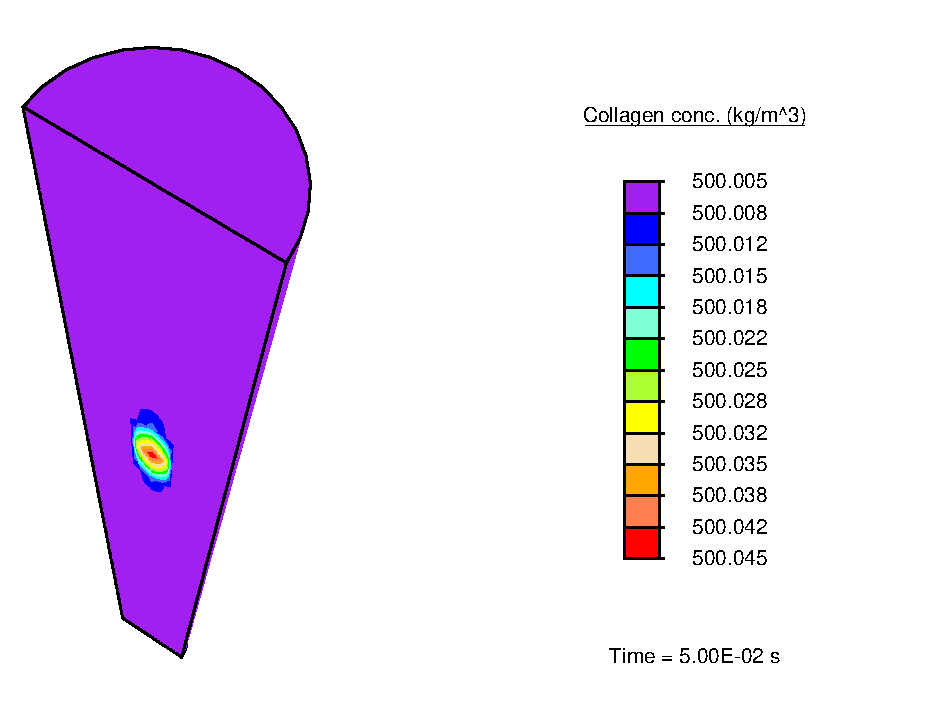
\includegraphics[width=0.8\textwidth]{images/examples/lagrangian/medication/final-collagen-concentration}
\caption{The collagen concentration (kg.m$^{-3}$) at time
  $t=5\times10^{-2}$~s.}
\label{eg3conc}
\end{figure}

This example incorporates all of the theory discussed in
Chapter~\ref{lagrangian-perspective}. However, it is a valuable
exercise in modelling to simplify the boundary value problem, and
suppress some of the coupled phenomena in order to gain a better
understanding of some effects. This is the approach followed in the
next two numerical examples. The detailed transport and mechanics
induced by the constrictive radial load are discussed first in
Section~\ref{constriction-1}.

\section{Examples exploring the biphasic nature of porous soft tissue}
\label{biphasic-examples-1}

In these calculations, only two phases---fluid and collagen---are
included for the mass transport and mechanics. As before, the
parameters used in the analysis are presented in
Table~\ref{parameters}.

\subsection{The tendon under constriction}
\label{constriction-1}

In this example, the tendon immersed in a bath is subjected to the
same constrictive radial load as in
Section~\ref{enzyme-kinetics-example}. Since that example demonstrated
an insignificant amount of local collagen production over this time
scale, we work with a simplified problem by setting the source term
$\Pi^\mathrm{c} = 0$. The total duration of the simulation is 10~s,
and the radial strain is applied as a displacement boundary condition,
increasing linearly from no strain initially to the maximum strain at
time $t = 1~\mathrm{s}$. Again, both the initial collagen
concentration and the initial fluid concentration are 500~kg.m$^{-3}$
at every point in the tendon. This tendon is exposed to a bath where
the fluid concentration is 500~kg.m$^{-3}$.

As mentioned in Section~\ref{computational-model}, when solving the balance of momentum
for the biphasic problem of the solid collagen and a fluid phase, the
tissue is currently treated as a single entity, employing a summation
of Equation~(\ref{localbalanceofmomentum}) over both species. Additionally,
condition~(\ref{momentumsummationresult}) allows us to avoid constitutive
prescription of the momentum transfer terms between solid collagen and
fluid phases,
$\bq^\mathrm{c}$ and $\bq^\mathrm{f}$. This facilitates considerable
simplification of the 
problem, but such a treatment requires additional assumptions on the
detailed deformation of the constitutive phases of the tissue.

\begin{figure}[!hpt]
  \centering
  \psfrag{A}{$\Omega_0$}
  \psfrag{B}{$\Omega_t$}
  \psfrag{C}{$\bF$}
  \psfrag{S}{\small Solid, `c'}
  \psfrag{F}{\small Fluid, `f'}
  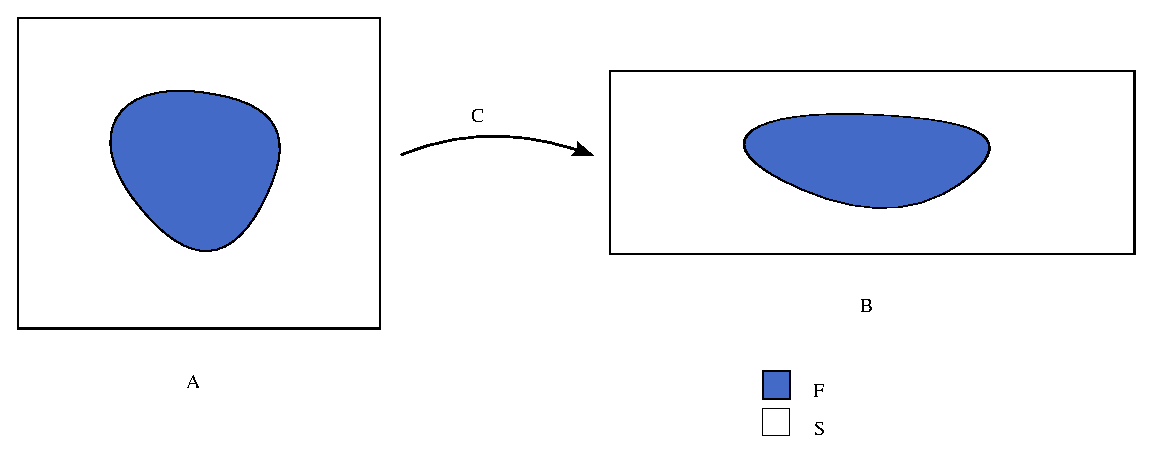
\includegraphics[width=0.8\textwidth]{images/elucidation/homogeneous-deformation}
  \caption{Upper-bound model from strain homogenisation.}
  \label{upper-bound-model}
\end{figure}

An implicit assumption we have drawn on thus far is the equality of
the deformation gradient of the solid collagen and pore spaces,
allowing us to use the deformation gradient $\bF$, suitably decomposed
to account for change in fluid concentration, to model the fluid
stress. This assumption, depicted in Figure~\ref{upper-bound-model},
had important consequences for the developments in Sections
\ref{balance-of-mass}, \ref{kinematics-of-growth},
\ref{saturation-and-tissue-swelling}, \ref{ideal-incompressible-fluid},
\ref{caviation-under-tension} and \ref{incompressible-fluid-porous-solid}.

Since the imposition of a common deformation gradient results in an
upper bound for the effective stiffness of the tissue and magnitudes
of the fluxes established, we refer to it as the {\em upper bound
  model}. This assumption plays a fundamental role in determining the
fluid flux driven by the fluid stress gradient.

\begin{figure}[!hpt]
  \centering
  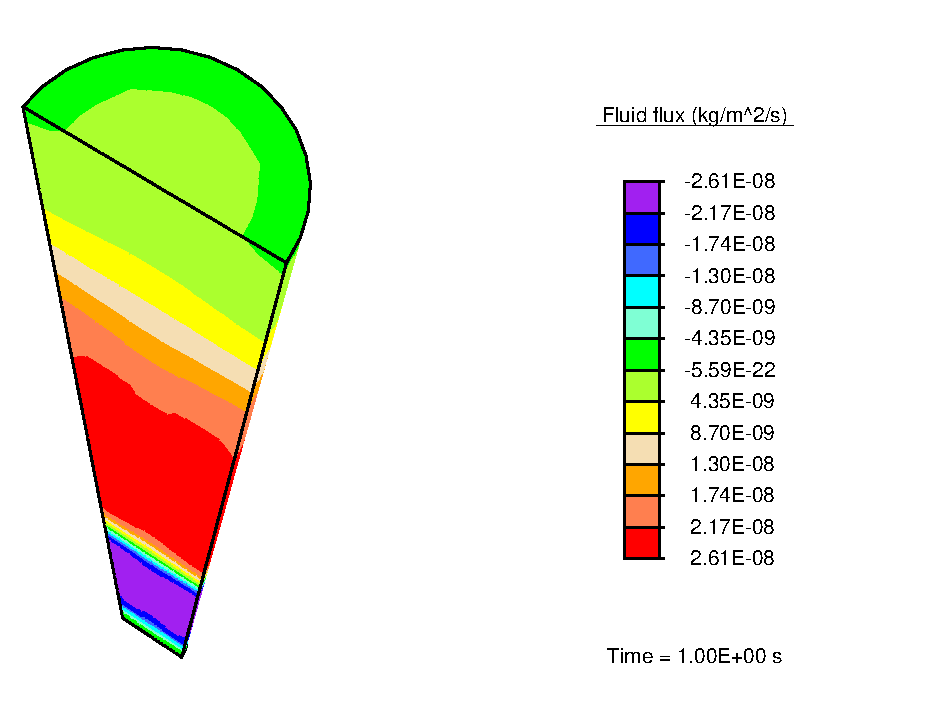
\includegraphics[width=0.8\textwidth]{images/examples/lagrangian/constriction/upper-bound-flux}
  \caption{{\em Upper bound} fluid flux (kg.m$^{-2}$.s$^{-1}$) in
    the vertical direction at time $t=1$~s.}
  \label{eg2flux}
\end{figure}

\noindent For this upper bound model, Figure~\ref{eg2flux} shows the
fluid flux in the vertical direction at the final stage of the
constriction phase of the simulation, i.e. at time $t=1$~s. The flux
values are positive above the central plane, forcing fluid upward, and
negative below, forcing fluid fluid downward. This stress-gradient
induced fluid flux results in a reference concentration distribution
of the fluid that is higher near the top and bottom faces, as seen in
Figure~\ref{eg2conc}.

\begin{figure}[!hpt]
  \centering
  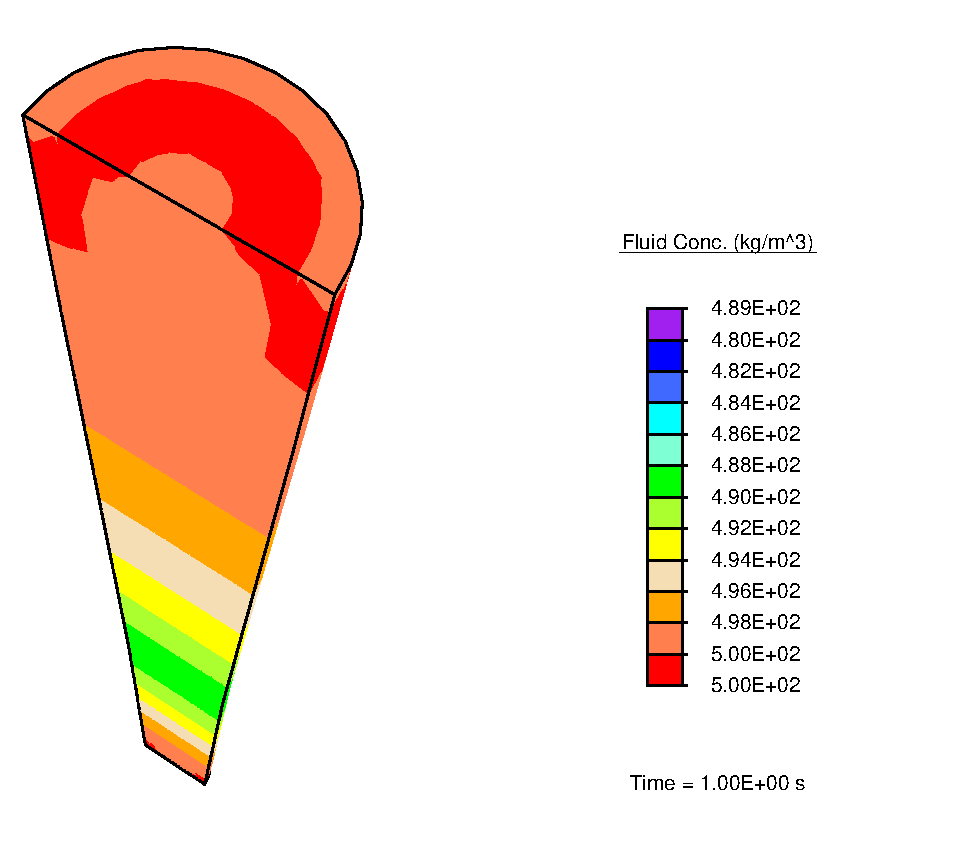
\includegraphics[width=0.8\textwidth]{images/examples/lagrangian/constriction/fluid-concentration}
  \caption{Reference fluid concentration (kg.m$^{-3}$) at time
    $t=1$~s.}
  \label{eg2conc}
\end{figure}

As a result, these regions would have seen a higher production of
collagen, or preferential growth, in the presence of non-zero source
terms. As discussed in Section~\ref{role-of-current-mass-balance}, the
mass transport equations are solved in the current configuration,
where physical boundary conditions can be set directly. The values
reported in Figure~\ref{eg2conc} are pulled back from the current
configuration. The current concentrations do not change for this
boundary value problem.

Solving a problem of this nature in the
reference configuration using $\rho_0^\mathrm{f} = $ const. as the
boundary condition to represent immersion of the tendon in a fluid bath
yields non-physical results, such as an unbounded flow. This occurs
since the imposed strain gradient causes a stress gradient in the
fluid that does not decay. The imposed boundary condition on $\rho_0^\mathrm{f}$
prevents a redistribution of concentration that would have provided an
opposing, internal gradient of stress, which in turn would drive the
flux to vanish.

% Todo: Perhaps the unbounded flow figures can be sneaked in around
% here.

The tendon is held fixed in the radial direction after the
constriction phase. The applied stress sets up a pressure wave in the
fluid travelling toward the top and bottom faces. As the fluid leaves
these surfaces, we observe that the tendon relaxes. This is seen in
Figure~\ref{topdisp}, which plots the vertical displacement of the top
face with time, showing a decrease in height of the tendon after the
constriction phase. We keep the centre of the bottom face of the
tendon fixed.

\begin{figure}[!hpt]
  \centering
      {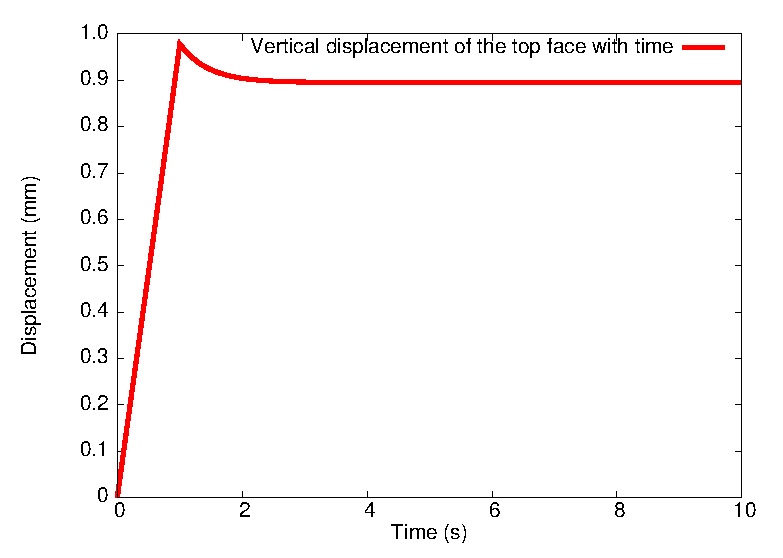
\includegraphics[width=0.8\textwidth]{images/examples/lagrangian/constriction/top-vertical-displacement}}
      \caption{Relaxation of the top face of the tendon after the
      constriction phase.}
      \label{topdisp}
\end{figure}

In order to define a range of the magnitude of fluid flux, we now
introduce the {\em lower bound model} (on effective stiffness of the
tissue and, consequently, the magnitude of the fluid flux). For this
lower bound, we replace the earlier strain homogenisation requirement
with a stress homogenisation requirement, {\em viz.} equating the
hydrostatic stress of the solid phase and the fluid pressure in the
current configuration:

\begin{equation}
p^{\mathrm{f}}=\frac{1}{3} \mathrm{\small{tr}}[\Bsigma^{c}],
\label{equalpr}
\end{equation}

\noindent where $p^{\mathrm{f}}$ is the fluid pressure in the current
configuration, $\mbox{\small{tr}[\textbullet]}$ is the trace operator, and
$\Bsigma^{c}=\frac{1}{\mathrm{J^{c}}} \bP^{\mathrm{c}}
\bF^{\mathrm{c}^{\mathrm{T}}}$ is the Cauchy stress of the solid. This
assumption is depicted in Figure~\ref{lower-bound-model}. The
Cauchy stress of an ideal fluid can be defined from its current
pressure as \mbox{$\Bsigma^{f}= p^{\mathrm{f}} \bone$.} 

\begin{figure}[ht]
  \centering
  \psfrag{A}{$\Omega_0$}
  \psfrag{B}{$\Omega_t$}
  \psfrag{C}{$\bF$}
  \psfrag{S}{\small Solid, `c'}
  \psfrag{F}{\small Fluid, `f'}
  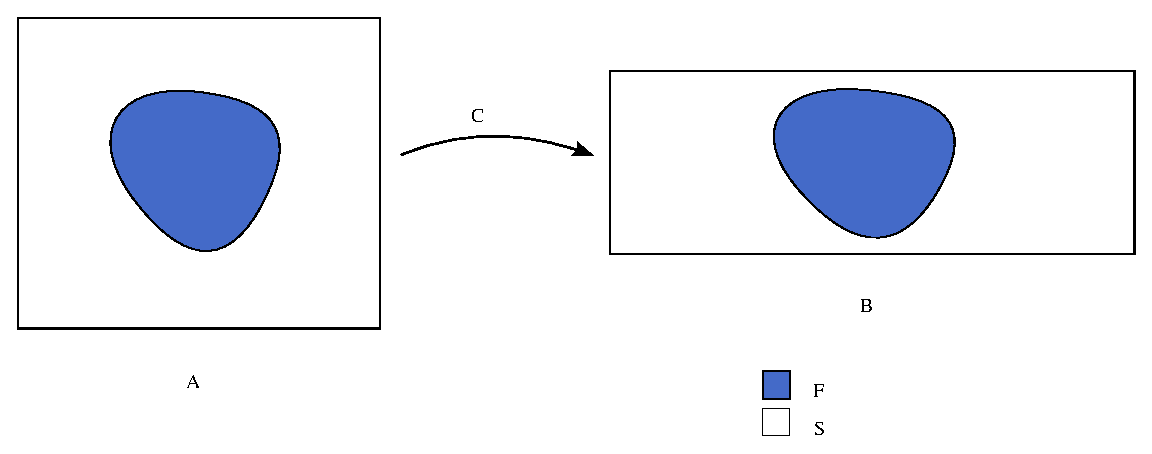
\includegraphics[width=0.8\textwidth]{images/elucidation/homogeneous-stress}
  \caption{Lower-bound model from stress homogenisation.}
  \label{lower-bound-model}
\end{figure}

Figure~{\ref{lowerbound}} reports the value of the vertical flux under
the lower bound modelling assumption, using boundary conditions identical to the
previous calculation at time $t=1$~s, the final stage of the
constriction phase of the simulation.

\begin{figure}[!hpt]
  \centering
      {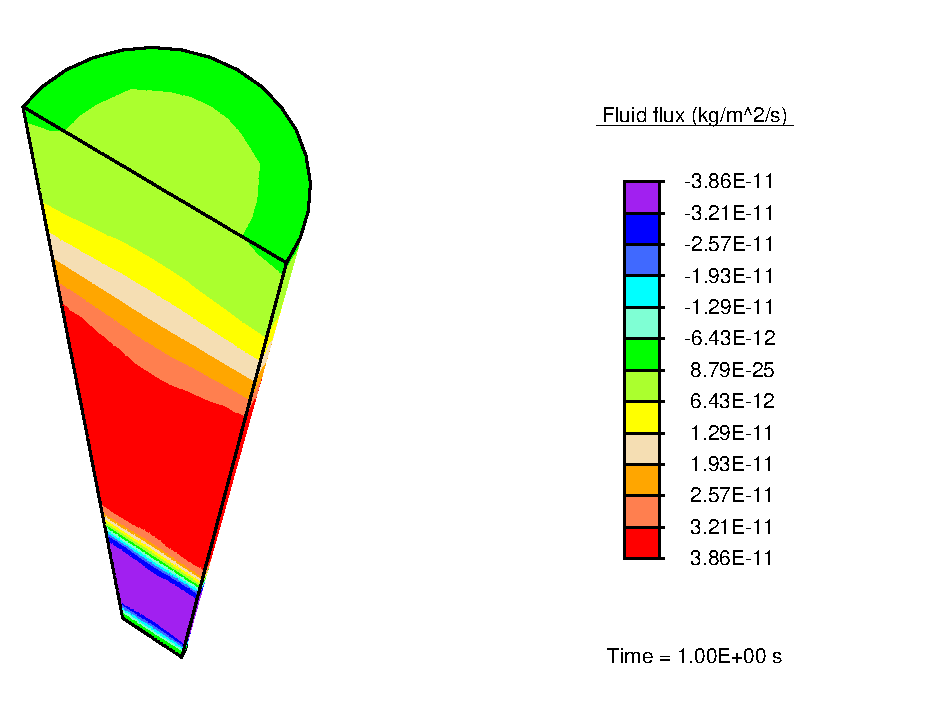
\includegraphics[width=0.8\textwidth]{images/examples/lagrangian/constriction/lower-bound-flux}}
      \caption{{\em Lower bound} fluid flux (kg.m$^{-2}$.s$^{-1}$) in
        the vertical direction at time $t=1$~s.}
      \label{lowerbound}
\end{figure}

The fluid flux values reported in Figures~\ref{eg2flux} and
\ref{lowerbound} (corresponding to the upper and lower bound modelling
assumptions, respectively) are qualitatively similar, but differ by
about three orders of magnitude.\footnote{The computational
  implementation used in Chapter~\ref{numerical-simulations-2} solves
  the detailed balance of momentum equations, i.e. a pushed-forward
  form of Equation~\ref{localbalanceofmomentum} for each species
  individually, obviating the need for either of these homogenisation
  assumptions.} This wide range points to the importance of imposing
the appropriate mechanical coupling model between interacting
phases. Note, however, that we now have the range of possible fluid
flux values under the specified mechanical loading. Recall,
furthermore, that the example in Section \ref{enzyme-kinetics-example}
used the upper bound model, and yet resulted in no discernible
advective solute transport. This suggests strongly that, given the
parameters in Table \ref{parameters}, convective transport of
nutrients in tendons is dominated by diffusive transport.

\begin{table}
\begin{center}
\begin{tabular}{|r|c|c|c|c|}
  \hline
  Pass & \multicolumn{2}{c|}{Strongly coupled} &
         \multicolumn{2}{c|}{Weakly coupled}\\
  \cline{2-5} & Residual & CPU (s) & Residual & CPU (s)\\
  \hline\hline 
1     & $ 2.138\times 10^{-02}$ &   29.16   & $6.761 \times 10^{-04}$  &    28.5 \\
      & $ 3.093\times 10^{-04}$ &   55.85   & $1.075 \times 10^{-04}$  &    55.1 \\
      & $ 2.443\times 10^{-06}$ &   82.37   & $4.984 \times 10^{-06}$  &    81.8 \\
      & $ 2.456\times 10^{-08}$ &  109.61   & $1.698 \times 10^{-08}$  &   107.9 \\
      & $ 4.697\times 10^{-14}$ &  135.83   & $3.401 \times 10^{-13}$  &   134.1 \\
      & $ 1.750\times 10^{-16}$ &  163.18   & $1.1523\times 10^{-17}$  &   161.1 \\
\hline                                    
2     & $ 5.308\times 10^{-06}$ &  166.79   & $5.971 \times 10^{-08}$  &  192.5  \\
      & $ 4.038\times 10^{-10}$ &  193.36   & $4.285 \times 10^{-11}$  &  218.6  \\
      & $ 1.440\times 10^{-14}$ &  220.45   & $2.673 \times 10^{-15}$  &  246.1  \\
      & $ 4.221\times 10^{-17}$ &  247.04   & $                    $   &  \\
\hline                                    
3     & $ 5.186\times 10^{-06}$ &  250.62   & $2.194 \times 10^{-09}$  &  277.3  \\
      & $ 3.852\times 10^{-10}$ &  277.44   & $2.196 \times 10^{-13}$  &  304.2   \\
      & $ 1.369\times 10^{-14}$ &  304.16   & $1.096 \times 10^{-17}$  &  331.6   \\
      & $ 4.120\times 10^{-17}$ &  331.47   & $                    $   &  \\
\hline                                    
4     & $ 5.065\times 10^{-06}$ &  335.16   & $8.160 \times 10^{-11}$  &  363.2 \\ 
      & $ 3.674\times 10^{-10}$ &  362.24   & $7.923 \times 10^{-15}$  &  390.2 \\
      & $ 1.300\times 10^{-14}$ &  388.79   & $                    $   &  \\
      & $ 4.021\times 10^{-17}$ &  416.08   & $                    $   &  \\
\hline                                    
5     & $ 4.948\times 10^{-06}$ &  419.59   & $3.078 \times 10^{-12}$  &  421.4 \\
      & $ 3.503\times 10^{-10}$ &  446.24   & $3.042 \times 10^{-16}$  &  448.6 \\
      & $ 1.236\times 10^{-14}$ &  473.20   & $                    $   &  \\
      & $ 3.924\times 10^{-17}$ &  500.85   & $                    $   &  \\
\hline                                    
6     & $ 4.832\times 10^{-06}$ &  504.65   & $1.179 \times 10^{-13}$  &  479.9 \\
      & $ 3.340\times 10^{-10}$ &  531.28   & $1.291 \times 10^{-17}$  &  507.0 \\
      & $ 1.174\times 10^{-14}$ &  558.17   & $                    $   &  \\
      & $ 3.829\times 10^{-17}$ &  585.27   & $                    $   &  \\
\hline                                    
7     & $ 4.720\times 10^{-06}$ &  589.01   & $4.592 \times 10^{-15}$  &  537.8 \\
      & $ 3.184\times 10^{-10}$ &  616.24   & $5.152 \times 10^{-18}$  &  564.6 \\
      & $ 1.116\times 10^{-14}$ &  643.29   & $                    $   &  \\
      & $ 3.737\times 10^{-17}$ &  670.83   & $                    $   &  \\
\hline                                    
8     & $ 4.609\times 10^{-06}$ &  674.46   & $1.816 \times 10^{-16}$  &  595.5  \\
      & $ 3.034\times 10^{-10}$ &  701.74   & $5.040 \times 10^{-18}$  &  622.3  \\
      & $ 1.060\times 10^{-14}$ &  727.74   & $                    $   &  \\
      & $ 3.646\times 10^{-17}$ &  755.58   & $                    $   &  \\
\hline
\end{tabular}
\caption{Mechanics equation residual norms.}
\label{resnorms}
\end{center}
{Mechanics equation residual norms and corresponding CPU times in
  seconds for the first 8 passes of each of the two cases for a
  typical time increment, \mbox{$\Delta t=0.1$ s}.}
\end{table}

This numerical example also points to the fact that a convenient
measure of the strength of coupling between the mechanics and mass
transport equations is the ratio of the variation in hydrostatic
stress of the fluid to that of the solid. In the lower bound case,
where the fluid response is defined by Equation~(\ref{equalpr}), it is
instructive to note that this ratio is unity. As a result, it is seen
that the lower bound case exhibits significantly weaker coupling than
the upper bound case. In the latter, variation in the common
deformation gradient, $\delta \bF$, causes instantaneous variation in
\mbox{$\delta p^{\mathrm{f}} \approx O(\kappa^{\mathrm{f}} \delta
  \bF:\bF^{-\mathrm{T}})$} and in \mbox{$\frac{1}{3}
  \delta\mathrm{\small{tr}}[\Bsigma^{c}] \approx O(\kappa^{\mathrm{c}}
  \delta \bF:\bF^{-\mathrm{T}})$}, where $\kappa^{\mathrm{c}}$ is the
bulk modulus of the solid. The ratio $\frac{\delta
  p^{\mathrm{f}}}{\frac{1}{3} \delta
  \mathrm{\small{tr}}[\Bsigma^{c}]}$ is therefore \mbox{$\approx
  O(\kappa^{\mathrm{f}}/\kappa^{\mathrm{c}}) \gg 1$}.

The strength of coupling between the equations plays a principal role
in the rate of convergence of the solution, as observed in
Table~\ref{resnorms}, where the residual norms of the equilibrium
equation (and corresponding CPU times in seconds for an
\mbox{Intel\textregistered\ Xeon} 3.4 GHz machine) are reported for the first
8 iterations of each of the two cases. Recall that the staggered
scheme involves solution of the mechanics equation keeping the
concentrations fixed, and the mass transport equation keeping the
displacements fixed, in turn, until the solution converges. The table
does not report the value of the residual norms arising from the
solution of the mass transport equation for the fluid, which occurs
after each reported solve of the of the mechanics equation. Although
the initial mechanics residual norms in successive passes are
decreasing linearly in both cases, the rapid decrease in this quantity
in the weakly-coupled case ensures convergence in far fewer iterations
than the strongly coupled case. Thus, the corresponding CPU times
reported are also lower for the weakly coupled case. This is
advantageous. In addition to being more physical, as argued at the
beginning of Section \ref{swelling-1} immediately below, the lower
bound, weakly-coupled case makes it feasible to drive problems to
longer, physiologically-relevant time-scales through the use of larger
time steps.



\subsection{A swelling problem}
\label{swelling-1}

Motivated mainly by the recognition that the lower bound model for
solid-fluid mechanical coupling ensures convergence to a
self-consistent solution in just a few passes of the staggered
solution scheme, it is used in subsequent examples in this chapter.

Note that the individual balance of linear momentum equations for the
solid collagenous and fluid phases with the momentum transfer terms
($\bq^\mathrm{c}, \bq^\mathrm{f}$ in (\ref{localbalanceofmomentum}))
is a statement of momentum balance between them. There is reason to
suppose, therefore, that equating the solid collagen and fluid stress,
or some component of these tensors as done in the lower bound model,
is a reasonable approximation to explicitly solving the balance of
linear momentum for each phase, including the momentum transfers. In
contrast, equating the deformation gradient of the solid collagen with
deformation of the pore spaces subjects the fluid to a stress state
also determined by this deformation gradient in the upper bound
model. This approximation does not correspond to an underlying
physical principle comparable to the satisfaction of individual
balances of linear momentum for solid collagen and fluid, with
momentum transfers. It is therefore somewhat less motivated and more
questionable. Clearly, a rigorous analysis or numerical comparisons of
all three models: upper bound, lower bound and direct solution of
individual solid-fluid momentum balances, must be carried out to
conclusively demonstrate this.

In this example we study the mechanical effects of growth due to
collagen production. In the interest of focusing on this issue, we
assume that fibroblasts are available, and that the fluid phase bears
the necessary nutrients for collagen production dissolved at a
suitable, constant concentration. Collagen production is assumed to be
governed by a first-order rate law, as discussed in
Section~\ref{nature-of-sources} (\romannumeral 1). In this calculation, the
reaction rate, $k^\mathrm{f}$, taken to be 0.07 $\mathrm{s}^{-1}$.

The boundary conditions in this example correspond to immersion of the
tendon in a nutrient-rich bath. The initial collagen concentration is
500~kg.m$^{-3}$ and the fluid concentration is 400~kg.m$^{-3}$ at
every point in the tendon. When this tendon is exposed to a bath
where the fluid concentration is 410~kg.m$^{-3}$,
i.e. $\rho^\mathrm{f}(\bx,t)=410~\mathrm{kg.m}^{-3} \forall \bx \in
\partial\Omega_t$, nutrient-rich fluid is transported into the tissue,
due to the pressure difference, induced by the concentration
difference, between the fluid in the tendon and in 
the bath (fluid stress gradient-driven flux). Thereby, the nutrient
concentration is elevated, leading to collagen production, fluid
consumption and, eventually, growth due to additional collagen. 

\begin{figure}[!hpt]
  \centering
  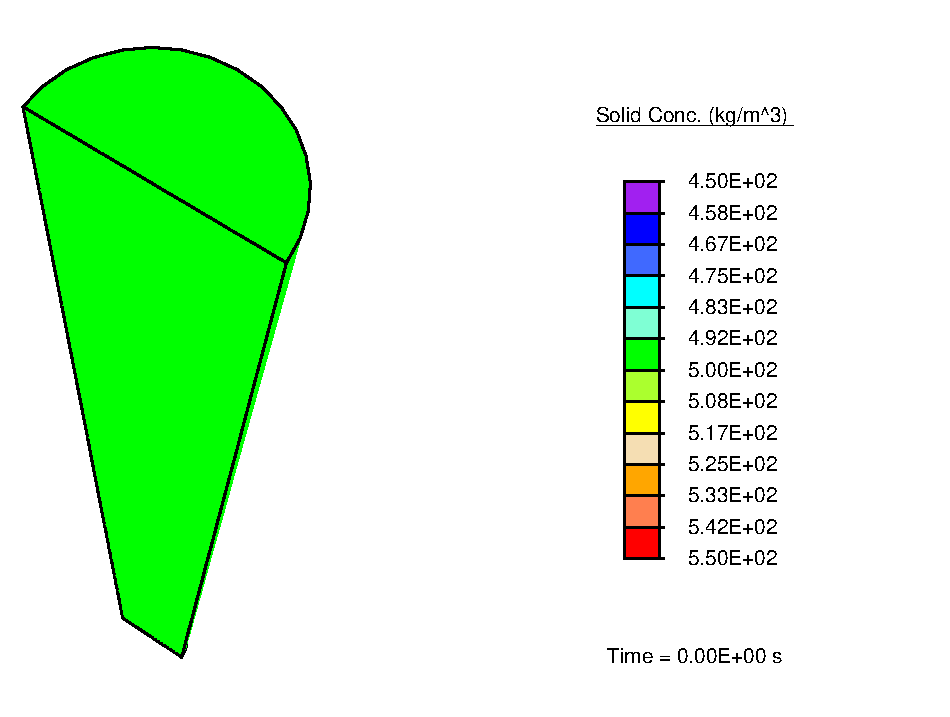
\includegraphics[width=0.8\textwidth]{images/examples/lagrangian/swelling/before-growth}
  \caption{The initial collagen concentration (kg.m$^{-3}$).}
  \label{before_growth}
\end{figure}

\begin{figure}[!hpt]
  \centering
  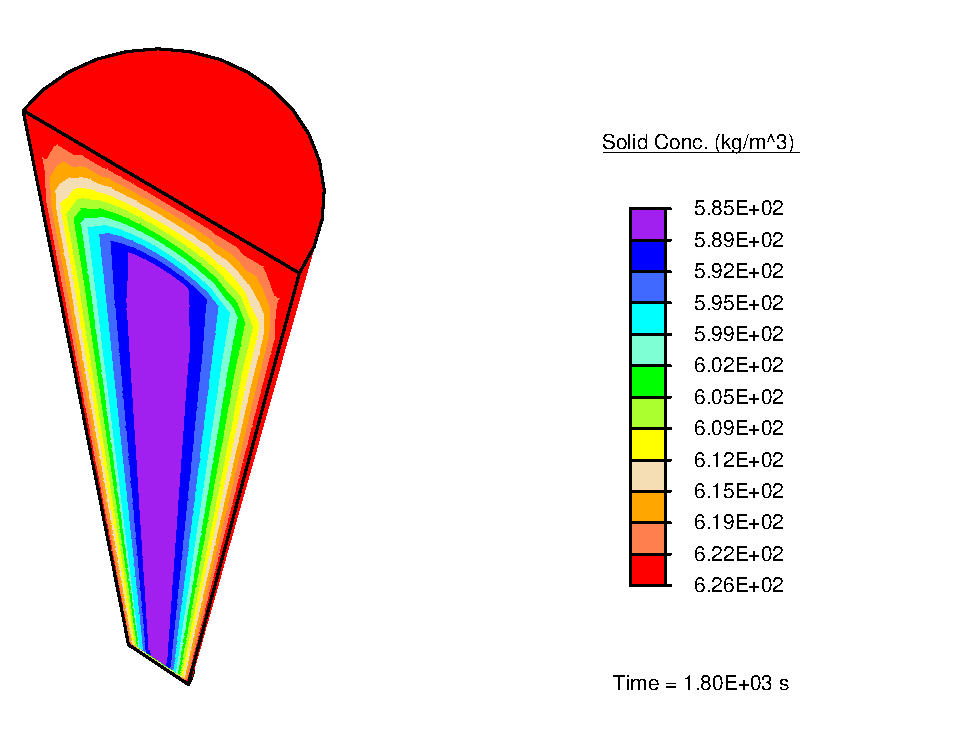
\includegraphics[width=0.8\textwidth]{images/examples/lagrangian/swelling/after-growth}
  \caption{The collagen concentration (kg.m$^{-3}$) after 1800~s.}
  \label{after_growth}
\end{figure}

Figure~\ref{before_growth} shows the initial collagen concentration in
the tendon. After it has been immersed in the nutrient-rich bath for
1800~s, the tendon shows growth and the collagen concentration is
higher as seen in Figure~\ref{after_growth}. On performing a uniaxial
tension test on the tendon before and after growth, it is observed
(Figure~\ref{stress_strain}) that the grown tissue is stiffer and
stronger due to its higher collagen concentration. Also note that
there is a rapid, fluid transport-dominated swelling of the tendon
between 0 and 25 s following immersion in the fluid bath
(Figure~\ref{volume_evolution}). This causes a small volume change of
$\approx 1.6$\%. In this transport-dominated regime the contribution
to tendon growth from collagen production is small. However, the
fluid-induced swelling saturates, and between 25 and 1800 s the
reaction producing collagen dominates the growth process, producing a
further $\approx 6.8$\% volume change. Noting that the range of
collagen concentration in Figure~\ref{after_growth} is $585-626\;
\mbox{kg.m}^{-3}$, and that (\ref{isotropicgrowth}) gives
$\bF^{\mathrm{g}^\mathrm{c}} = \left(
\frac{\rho_0^\mathrm{c}}{\rho_{0_{\mathrm{ini}}}^\mathrm{c}} \right)^
     {\frac{1}{3}} {\bf 1}$, this portion of the volume change is
     quite clearly due to collagen production. The total volume change
     of $8.4$\% corresponds to changes in each linear dimension of the
     tendon by only $\approx 2.7$\%, and is not discernible upon
     comparing Figures~\ref{before_growth} and \ref{after_growth}. It
     is, however, manifest in Figure~\ref{volume_evolution}.

\begin{figure}[!hpt]
  \centering
  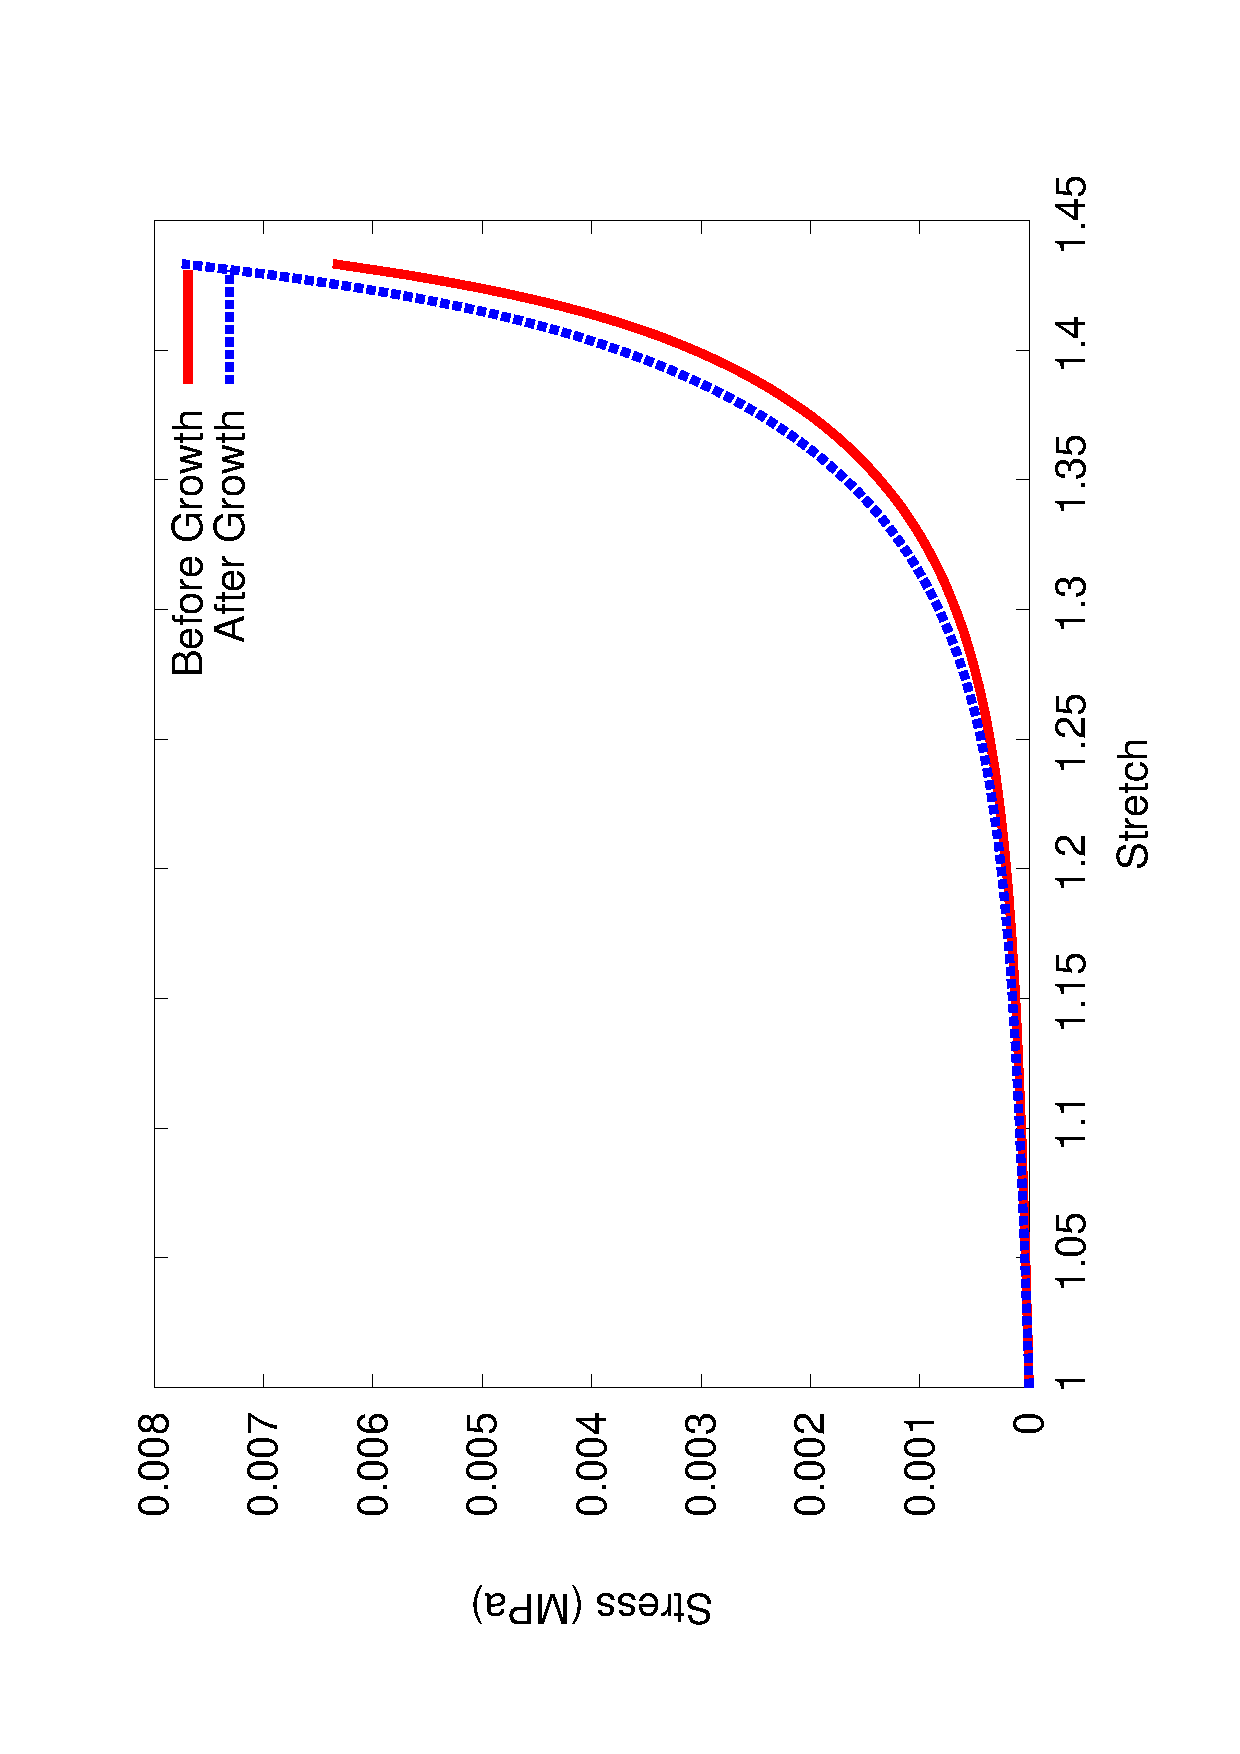
\includegraphics[angle=270,width=0.8\textwidth]{images/examples/lagrangian/swelling/stress-stretch}
  \caption{The stress (Pa) vs stretch curves before and after growth.}
  \label{stress_strain}
\end{figure}

\begin{figure}[!hpt]
  \begin{center}
    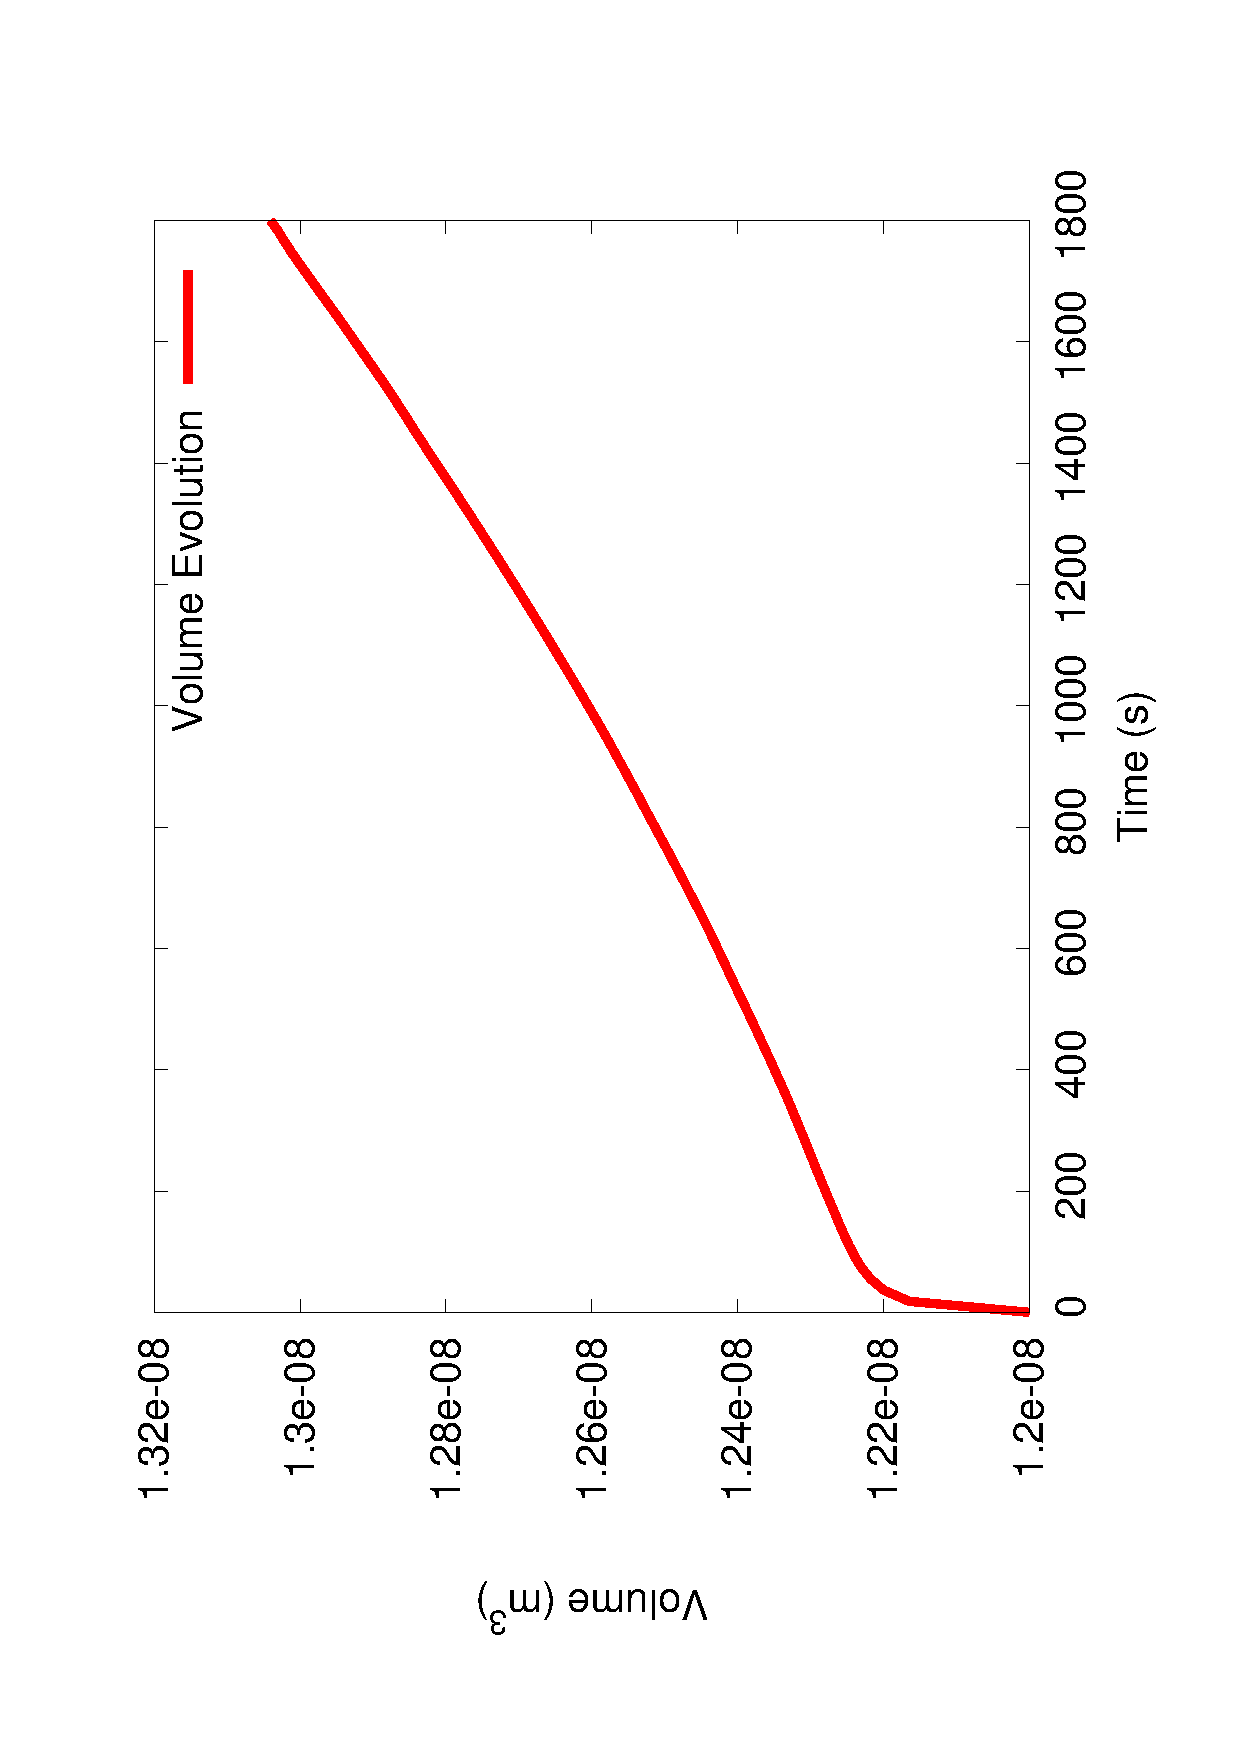
\includegraphics[angle=270,width=0.8\textwidth]{images/examples/lagrangian/swelling/volume-evolution-3}
    \caption{The volume of the tendon (m$^3$) evolving with
      time.}
    \label{volume_evolution}
  \end{center}
  {Note the fluid transported-dominated regime until 25 s,
    followed by the longer reaction-dominated growth stage.}
\end{figure}


%% \begin{figure}[!hpt]
%% \centering
%% 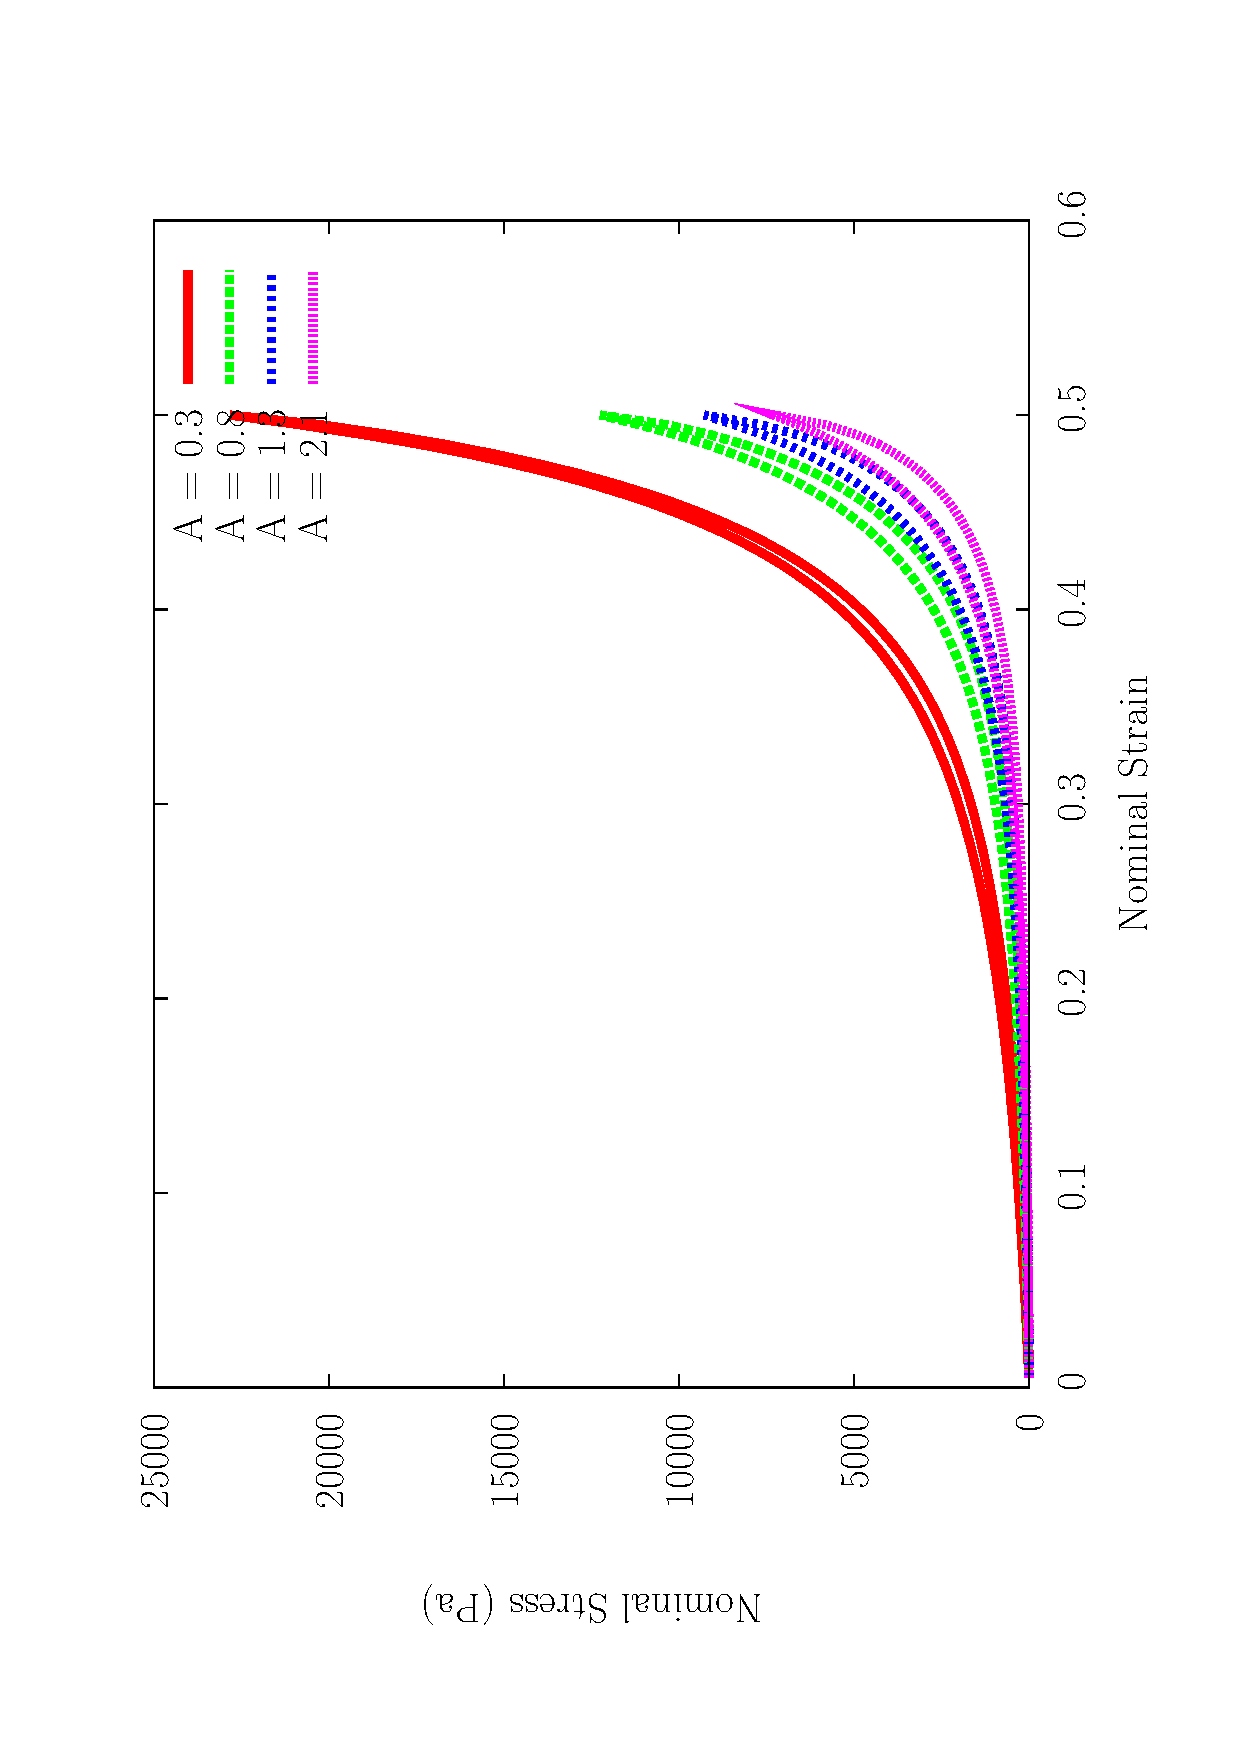
\includegraphics[angle=270,width=0.6\textwidth]{images/examples/lagrangian/cyclic/parametric-study}
%% \caption{Varying A}
%% \label{parametric-study}
%% \end{figure}

%% \begin{figure}[!hpt]
%% \centering
%% 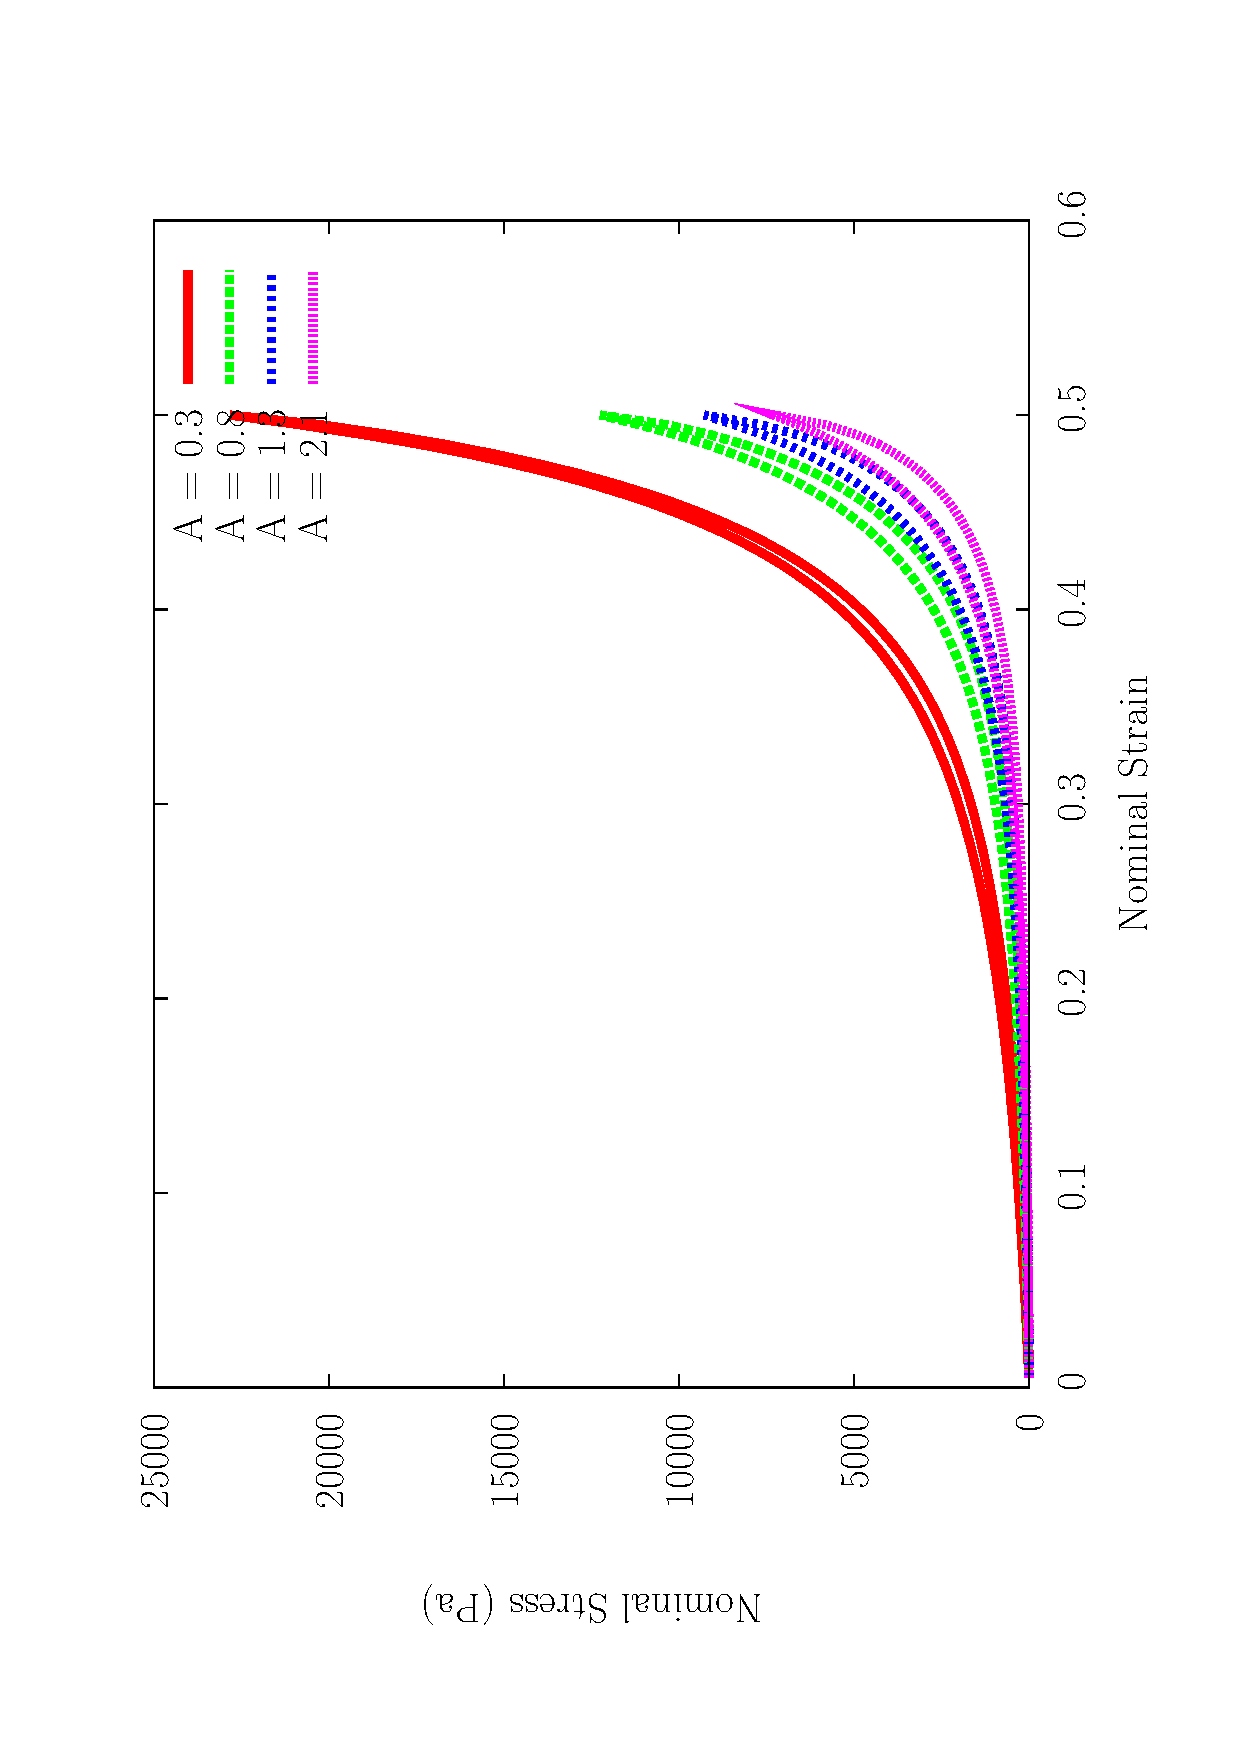
\includegraphics[angle=270,width=0.6\textwidth]{images/examples/lagrangian/cyclic/parametric-study}
%% \caption{Load-unload cycle}
%% \label{cyclic-load}
%% \end{figure}

\section{Extension to modelling wound healing}
\label{wound-healing-example}

%of scars are the result of the body overproducing collagen, which causes the scar to be raised above the surrounding skin. Hypertrophic scars take the form of a red raised lump on the skin, but do not grow beyond the boundaries of the original wound, and they often improve in appearance after a few years

%% chemo-mechanical
%% coupling is described in \cite{Provenzanoetal:2003}.

\begin{figure}[!hpt]
\centering
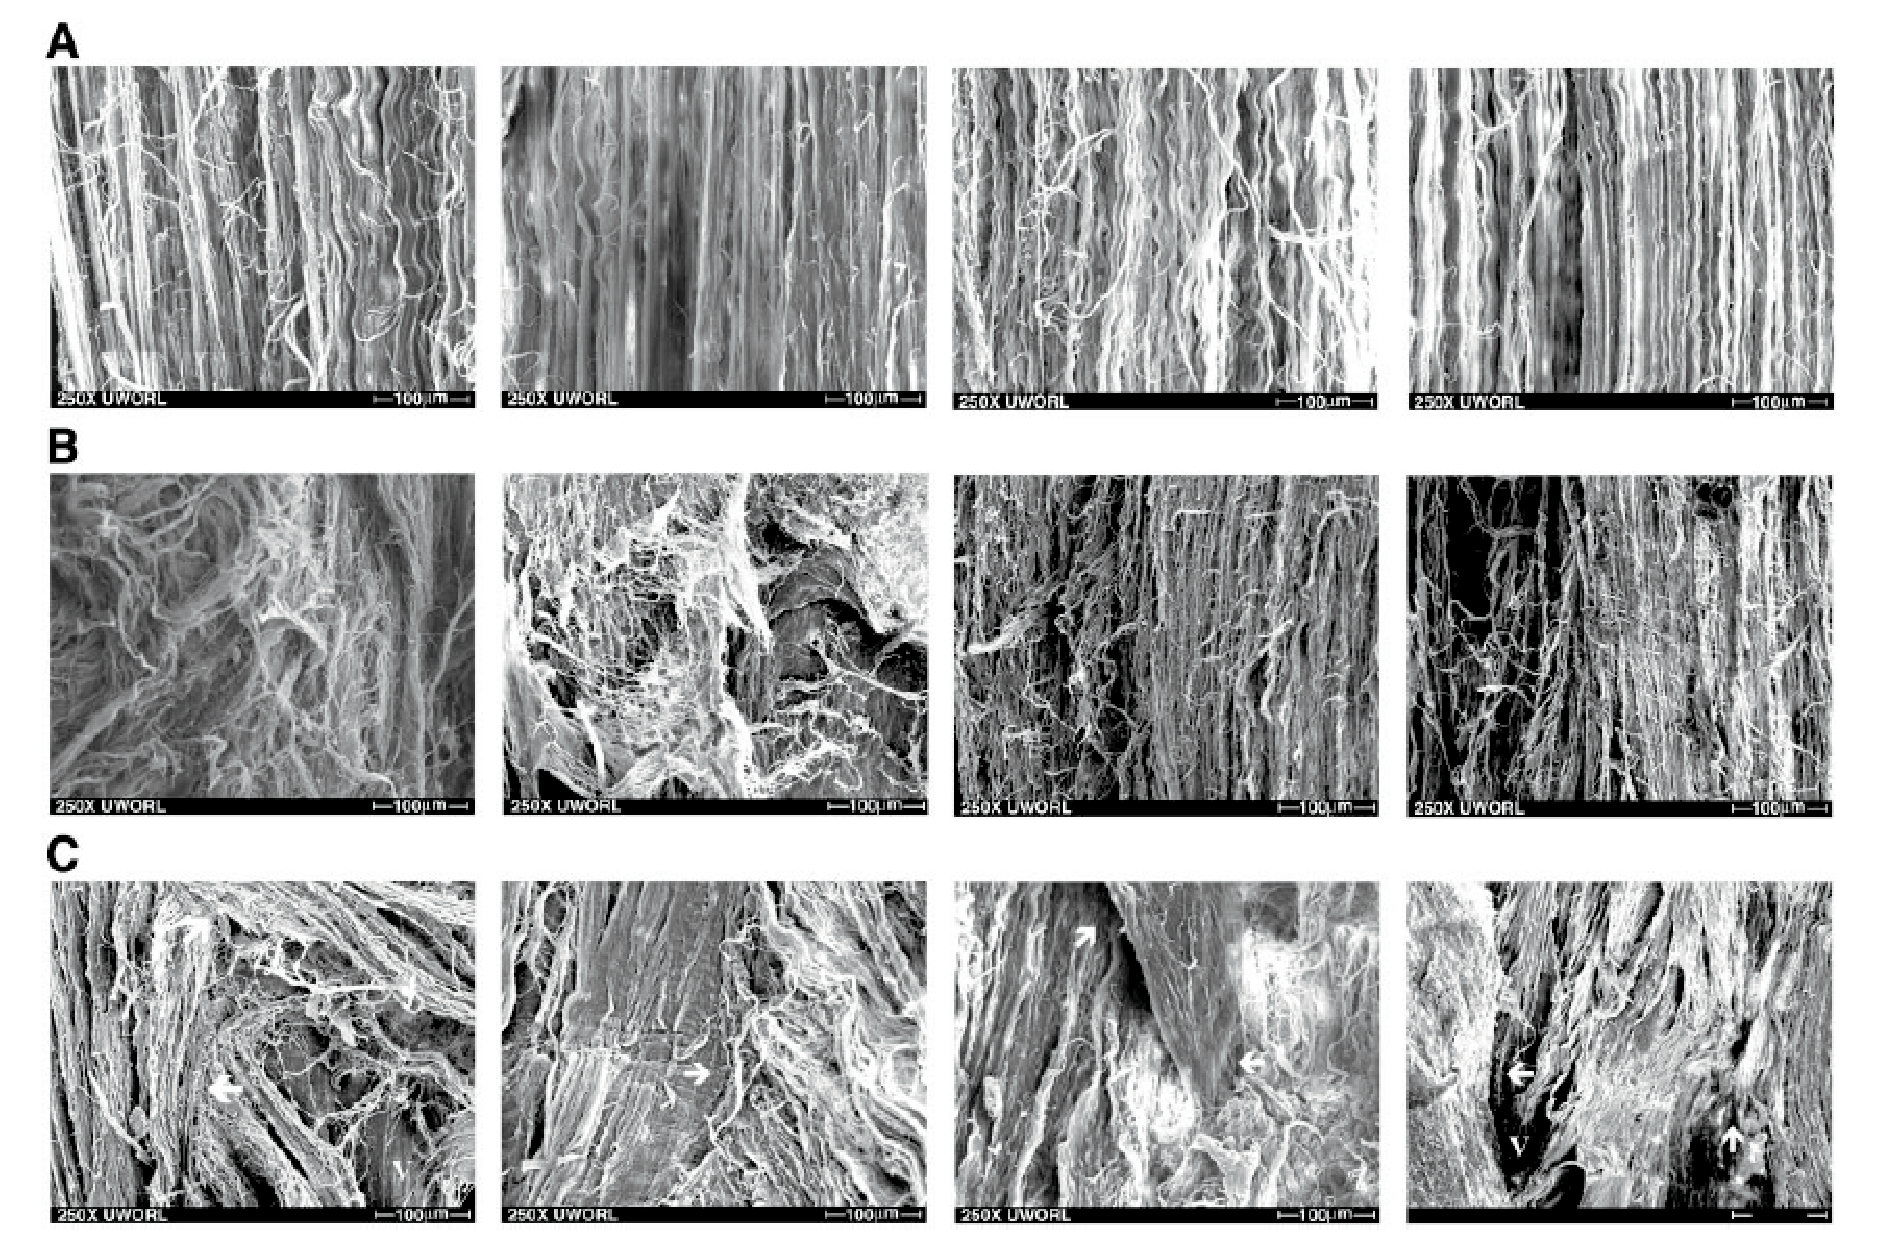
\includegraphics[width=0.8\textwidth]
                {images/experiments/healing-damaged-ligament} 
\caption{The recovery of a damaged ligament.}
\label{healing-damaged-ligament}
\end{figure}

\begin{figure}[!hpt]
\centering
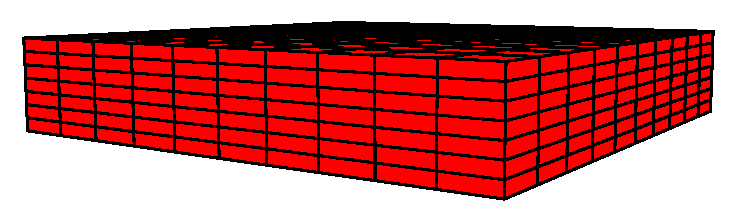
\includegraphics[width=0.8\textwidth]
                {images/examples/lagrangian/healing/full-skin-mesh} 
\caption{The computational mesh representing skin.}
\label{healing-skin-mesh}
\end{figure}

\begin{figure}[!hpt]
\centering
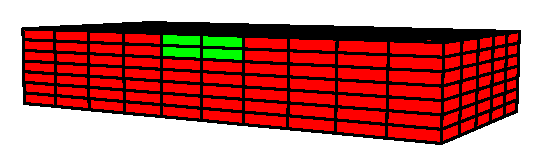
\includegraphics[width=0.8\textwidth]
                {images/examples/lagrangian/healing/damaged-region} 
\caption{The damaged region of the skin highlighted.}
\label{healing-damaged-region}
\end{figure}

\begin{figure}[!hpt]
\centering
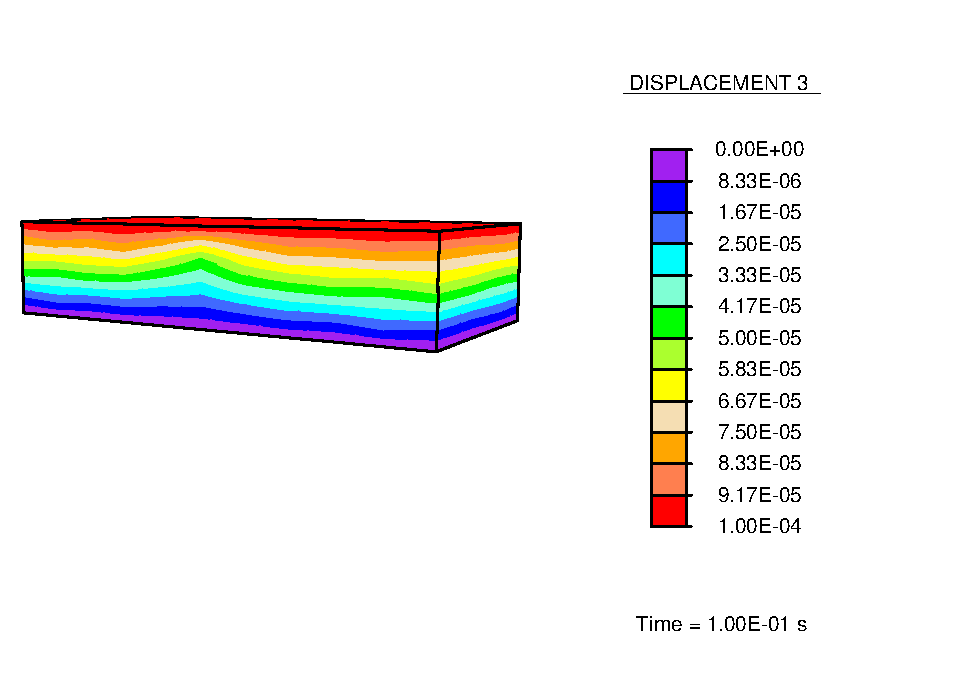
\includegraphics[width=0.8\textwidth]
                {images/examples/lagrangian/healing/healed-vertical-displacement} 
\caption{Vertical displacement upon loading after healing under no external load.}
\label{healing-vertical-displacement}
\end{figure}

\begin{figure}[!hpt]
\centering
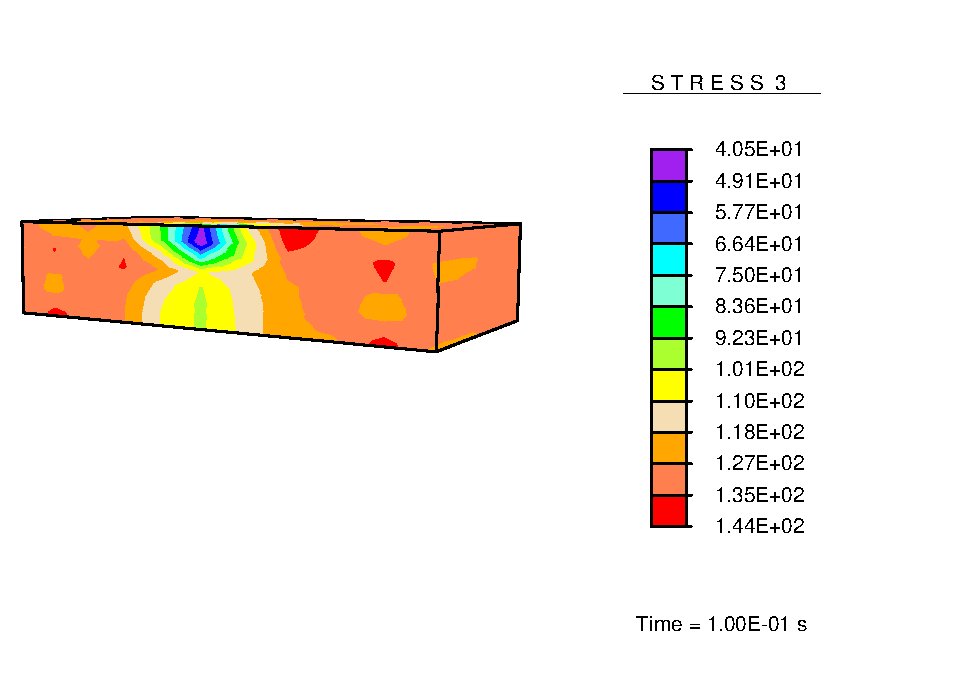
\includegraphics[width=0.8\textwidth]
                {images/examples/lagrangian/healing/healed-vertical-stress} 
\caption{Vertical stress upon loading after healing under no external load.}
\label{healing-vertical-stress}
\end{figure}

%% \todo{\begin{itemize}
%%   \item Stronger after growth and mechanics can go here; the tendon
%%     picture can go to the introduction.
%%   \item Needs some literature on the wound healing example; refer
%%     talk10.pdf.
%%   \item Weave around computational details yet again. Point to
%%     established, well known methods of solving the equations and point
%%     to the previous chapter's this-thesis-specific enhancements.
%% \end{itemize}}

%

% Local Variables:
% TeX-master: "thesis"
% mode: latex
% mode: flyspell
% End:
